% !TeX root = RJwrapper.tex
\title{The R Package \pkg{HDSpatialScan} for the Detection of Clusters of Multivariate and Functional Data using Spatial Scan Statistics}
\author{by Camille Frévent, Mohamed-Salem Ahmed, Julien Soula, Zaineb Smida, Lionel Cucala, Sophie Dabo-Niang and Michaël Genin}

\maketitle

\abstract{
This paper introduces the R package \CRANpkg{HDSpatialScan}. This package allows users to easily apply spatial scan statistics to real-valued multivariate data or both univariate and multivariate functional data. It also permits plotting the detected clusters and to summarize them. In this article the methods are presented and the use of the package is illustrated through examples on environmental data provided in the package.
}

% \section{Section title in sentence case}

% Introductory section which may include references in parentheses
% \citep{R}, or cite a reference such as \citet{R} in the text.

\section{Introduction} \label{sec:intro}
Spatial cluster detection methods are useful tools for objective detection and localization of statistically significant aggregation of events indexed in space. Examples of the applications of these methods are numerous: in the field of epidemiology, these methods allow epidemiologists to detect spatial clusters of disease cases and to formulate etiological hypotheses; in the environmental sciences, researchers can be led to search for particularly polluted geographical areas, either by one pollutant in particular or by several pollutants simultaneously. In astronomy, researchers may want to identify star clusters from telescope image data.\\

\noindent Several cluster detection methods have been proposed in the literature. In particular, spatial scan statistics (originally proposed by \citet{spatialdisease} and \citet{spatialscanstat} for Bernoulli and Poisson models) are powerful methods for detecting statistically significant spatial clusters, which can be defined by an aggregation of sites presenting an abnormal concentration (mean, etc) of an observed variable, with a variable scanning window and in the absence of pre-selection bias (objective detection of the cluster). Following on from Kulldorff's initial work, several researchers have adapted spatial scan statistics to other spatial data distributions: exponential \citep{huang2007spatial},
ordinal \citep{jung2007spatial}, normal \citep{normalkulldorff}, Weibull \citep{bhatt2014spatial}, etc. Others use nonparametric approaches such as \citet{A_nonparametric_spatial} and \citet{cucala2016mann} who respectively extend the Wilcoxon-Mann-Whitney test for spatial scan statistics and for temporal or spatial scan statistics. Note that in the case of spatial data the two approaches are equivalent by generalizing the method of \citet{A_nonparametric_spatial} to detect either high or low clusters. \\

\noindent The applications of scan statistics are numerous. In the field of epidemiology, \citet{khan2021geographic} detected significant clusters of diabetes incidence in Florida between 2007 and 2010, which will help guide local health policies. \citet{marciano2018epidemiological} sought to detect spatial clusters of leprosy incidence in a hyperendemic Brazilian municipality between 2000 and 2005 and 2006 and 2010. The study showed a high percentage of contact between people which facilitates the transmission of the disease. %Improved sanitary conditions, as well as earlier diagnosis, could also be ways to curb the epidemic. 
\citet{genin2020fine} detected high-risk clusters of Crohn's disease in France over the period 2007-2014. As the causes of this disease are still poorly understood, the detection of spatial clusters of Crohn's disease allows the researchers to make hypotheses on possible risk factors, such as high-social deprivation or high urbanization.
In the context of environmental science, the detection of clusters of symptomatic exposure to pesticides in rural areas \citep{sudakin2002regional} would allow the monitoring and prevention of pesticide-related diseases. \citet{geology} focused on the presence of iodine in drinking water in Shandong Province, China. The detection of spatial clusters of iodine presence in drinking water allows an improvement of the monitoring of drinking water quality in these geographical areas. Finally in the context of pollution data, \cite{wan2020industrial} and \cite{shi2021spatial} respectively detected clusters of high concentrations of $\text{PM}_{2.5}$ in America and China. Such results may allow local authorities to specifically monitor these areas and make decisions to reduce pollution. \\

\noindent When multiple variables are observed simultaneously at each spatial location, researchers may be interested in detecting spatial clusters with anomalous values of all measured variables. In this context, \citet{kulldorffmulti} proposed a multivariate spatial scan statistic using a combination of independent univariate scan statistics. However it fails to take into account the potential correlations between the variables. A first spatial scan statistic for multivariate data taking into account the correlations was proposed by \citet{a_multivariate_gaussian}. Their method is based on a multivariate normal probability model and a likelihood ratio. Later, \citet{nonparam_multi} proposed a nonparametric spatial scan statistic for multivariate data based on a multivariate Wilcoxon-Mann-Whitney test. \\ 

\noindent Technological developments in measurement tools and data storage capacity have yielded to the increasing use of sensors, cell phones and more generally connected devices that collect data continuously or almost continuously over time. 
This has led to the introduction of new analysis methods for functional data \citep{ramsaylivre}, as well as the adaptation of classical statistical methods such as principal component analysis \citep{fpc_boente, fpc_berrendero} or regression \citep{reg_cuevas, reg_ferraty, reg_chiou}. \\
\noindent In the field of spatial scan statistics, \citet{notre_fonctionnel} and \citet{wilco_cucala} proposed new methods for univariate processes. However for example, in environmental surveillance, numerous %continuous 
variables are simultaneously measured, making a multivariate functional approach necessary to detect environmental black-spots. These can be defined as geographical areas characterized by elevated concentrations of multiple pollutants. Although \citet{wilco_cucala} only studied their approach in the univariate functional framework, they suggest that it could also be adapted for multivariate processes. \citet{notre_fonctionnel1} studied this adaptation and also developed new efficient methods for multivariate functional spatial scan statistics. \\

\noindent In R several packages provide spatial scan statistics implementations. The best known is certainly the \CRANpkg{rsatscan} \citep{rsatscan} package which provides functions to interface R and the SaTScan software \citep{satscan}, allowing the latter to be launched from R.  
It implements lots of univariate methods (ordinal, Bernoulli, Poisson, \dots) but also the space-time spatial scan statistic \citep{space-time} and the multivariate extensions proposed by \citet{kulldorffmulti}. The function \code{kulldorff} implemented in the R package \CRANpkg{SpatialEpi} \citep{spatialepi} also performs the spatial scan statistics based on the Poisson and the Bernoulli models. Other softwares were created to detect clusters such as ClusterSeer \citep{clusterseer1, clusterseer2} which performs spatial, temporal and space-time clustering, and TreeScan \citep{treescan} which implements the tree-based scan statistic \citep{tree}. We should also mention the R package \CRANpkg{DCluster} \citep{DCluster} which implements the spatial scan statistics for Poisson or Bernoulli models. The R package \CRANpkg{DClusterm} \citep{JSSv090i14, Dclusterm} also implements a cluster detection method. Briefly, it consists in considering a large number of generalized linear models by including potential cluster indicators one by one, and then to use a model selection procedure.
The Shiny application SpatialEpiApp \citep{spatialepiapp1} and the R package \CRANpkg{SpatialEpiApp} \citep{SpatialEpiApp} allow the detection and visualization of clusters by using the scan statistics implemented in SaTScan.
Finally the software FlexScan \citep{flexscan} and the R package \CRANpkg{rflexscan} \citep{rflexscan} implement the spatial scan statistic using a scan window with a non pre-defined shape, defined by \citet{biv_power}. Other R packages also allow clusters detection such as \CRANpkg{graphscan} \citep{graphscan} (the \code{cluster} function), \pkg{SPATCLUS} \citep{spatclus} or \CRANpkg{scanstatistics} \citep{scanstatisticsman,scanstatistics} for spatial or space-time data. It should be noted that these last two packages are no longer available on the CRAN (The Comprehensive R Archive Network) repository. Although existing packages implement a large number of statistical spatial scan models, none of them propose multivariate scan models taking into account the potential correlations between variables or scan models for functional data. Thus, we have developed the R package \pkg{HDSpatialScan} for high-dimensional spatial scan statistics. The latter allows on the one hand the detection of spatial clusters in multivariate or functional data, and on the other hand, their display on a map and the description of their characteristics.


\noindent This paper is organized as follows: The following section presents the different models implemented in the R package \pkg{HDSpatialScan}. Then, the implementation of the methods is described and examples of use of the package are given. The last section concludes the paper.\\

\section{Models} \label{sec:method}

\noindent Let $s_1, \dots, s_n$ be $n$ different locations of an observation domain $S \subset \mathbb{R}^2$ and $X_1, \dots, X_n$ be the observations of a variable $X$ in $s_1, \dots, s_n$. Hereafter all observations are considered to be independent, which is a classical assumption in scan statistics. Three types of spatial data can be considered: either lattice data (the data  are aggregated at the spatial level, e.g.: county), geostatistical data (the variable is defined on a continuous area and each individual measure corresponds to a unique fixed spatial location, e.g.: pollutant concentration measured by sensors over a region), or marked point data (each individual measure corresponds to a unique random spatial location, e.g.: height of the trees in a forest, the location of the trees is random). 

\noindent Spatial scan statistics aim at detecting spatial clusters and testing their statistical significance. Hence, one tests a null hypothesis $\mathcal{H}_0$ (the absence of a cluster) against a composite alternative hypothesis $\mathcal{H}_1$ (the presence of at least one cluster $w \subset S$ presenting abnormal values of $X$). 
For this purpose, a spatial scan statistic consists of two steps. The first one is a detection phase using a scanning window of variable size and shape. We will focus here on the approach of \citet{spatialdisease} which use a circular scanning window of variable center and radius, however it should be noted that other shapes can be considered \citep{elliptic,cucala2013spatial}. An approach often advised is to limit the maximum size to half of the studied region since otherwise it would be like detecting a ``negative cluster'' in the areas outside the clusters covering almost all the studied region \citep{spatialdisease}. Then the scanning window allows to define a set of potential clusters $\mathcal{W}$ by
\begin{equation} \label{eq:cluster}
\mathcal{W} = \{ w_{i,j} \ / \ 1 \le |w_{i,j}| \le \frac{n}{2}, \ 1 \le i,j \le n \},
\end{equation}
where $w_{i,j}$ is the disc centered on $s_i$ that passes through $s_j$ and $|w_{i,j}|$ corresponds to the number of sites in $w_{i,j}$.
Figure~\ref{fig:potentialclusters} illustrates the set of potential clusters defined with a circular scanning window with Equation~\ref{eq:cluster} on a set of eight administrative areas in France.

\begin{figure}[htbp]
\centering
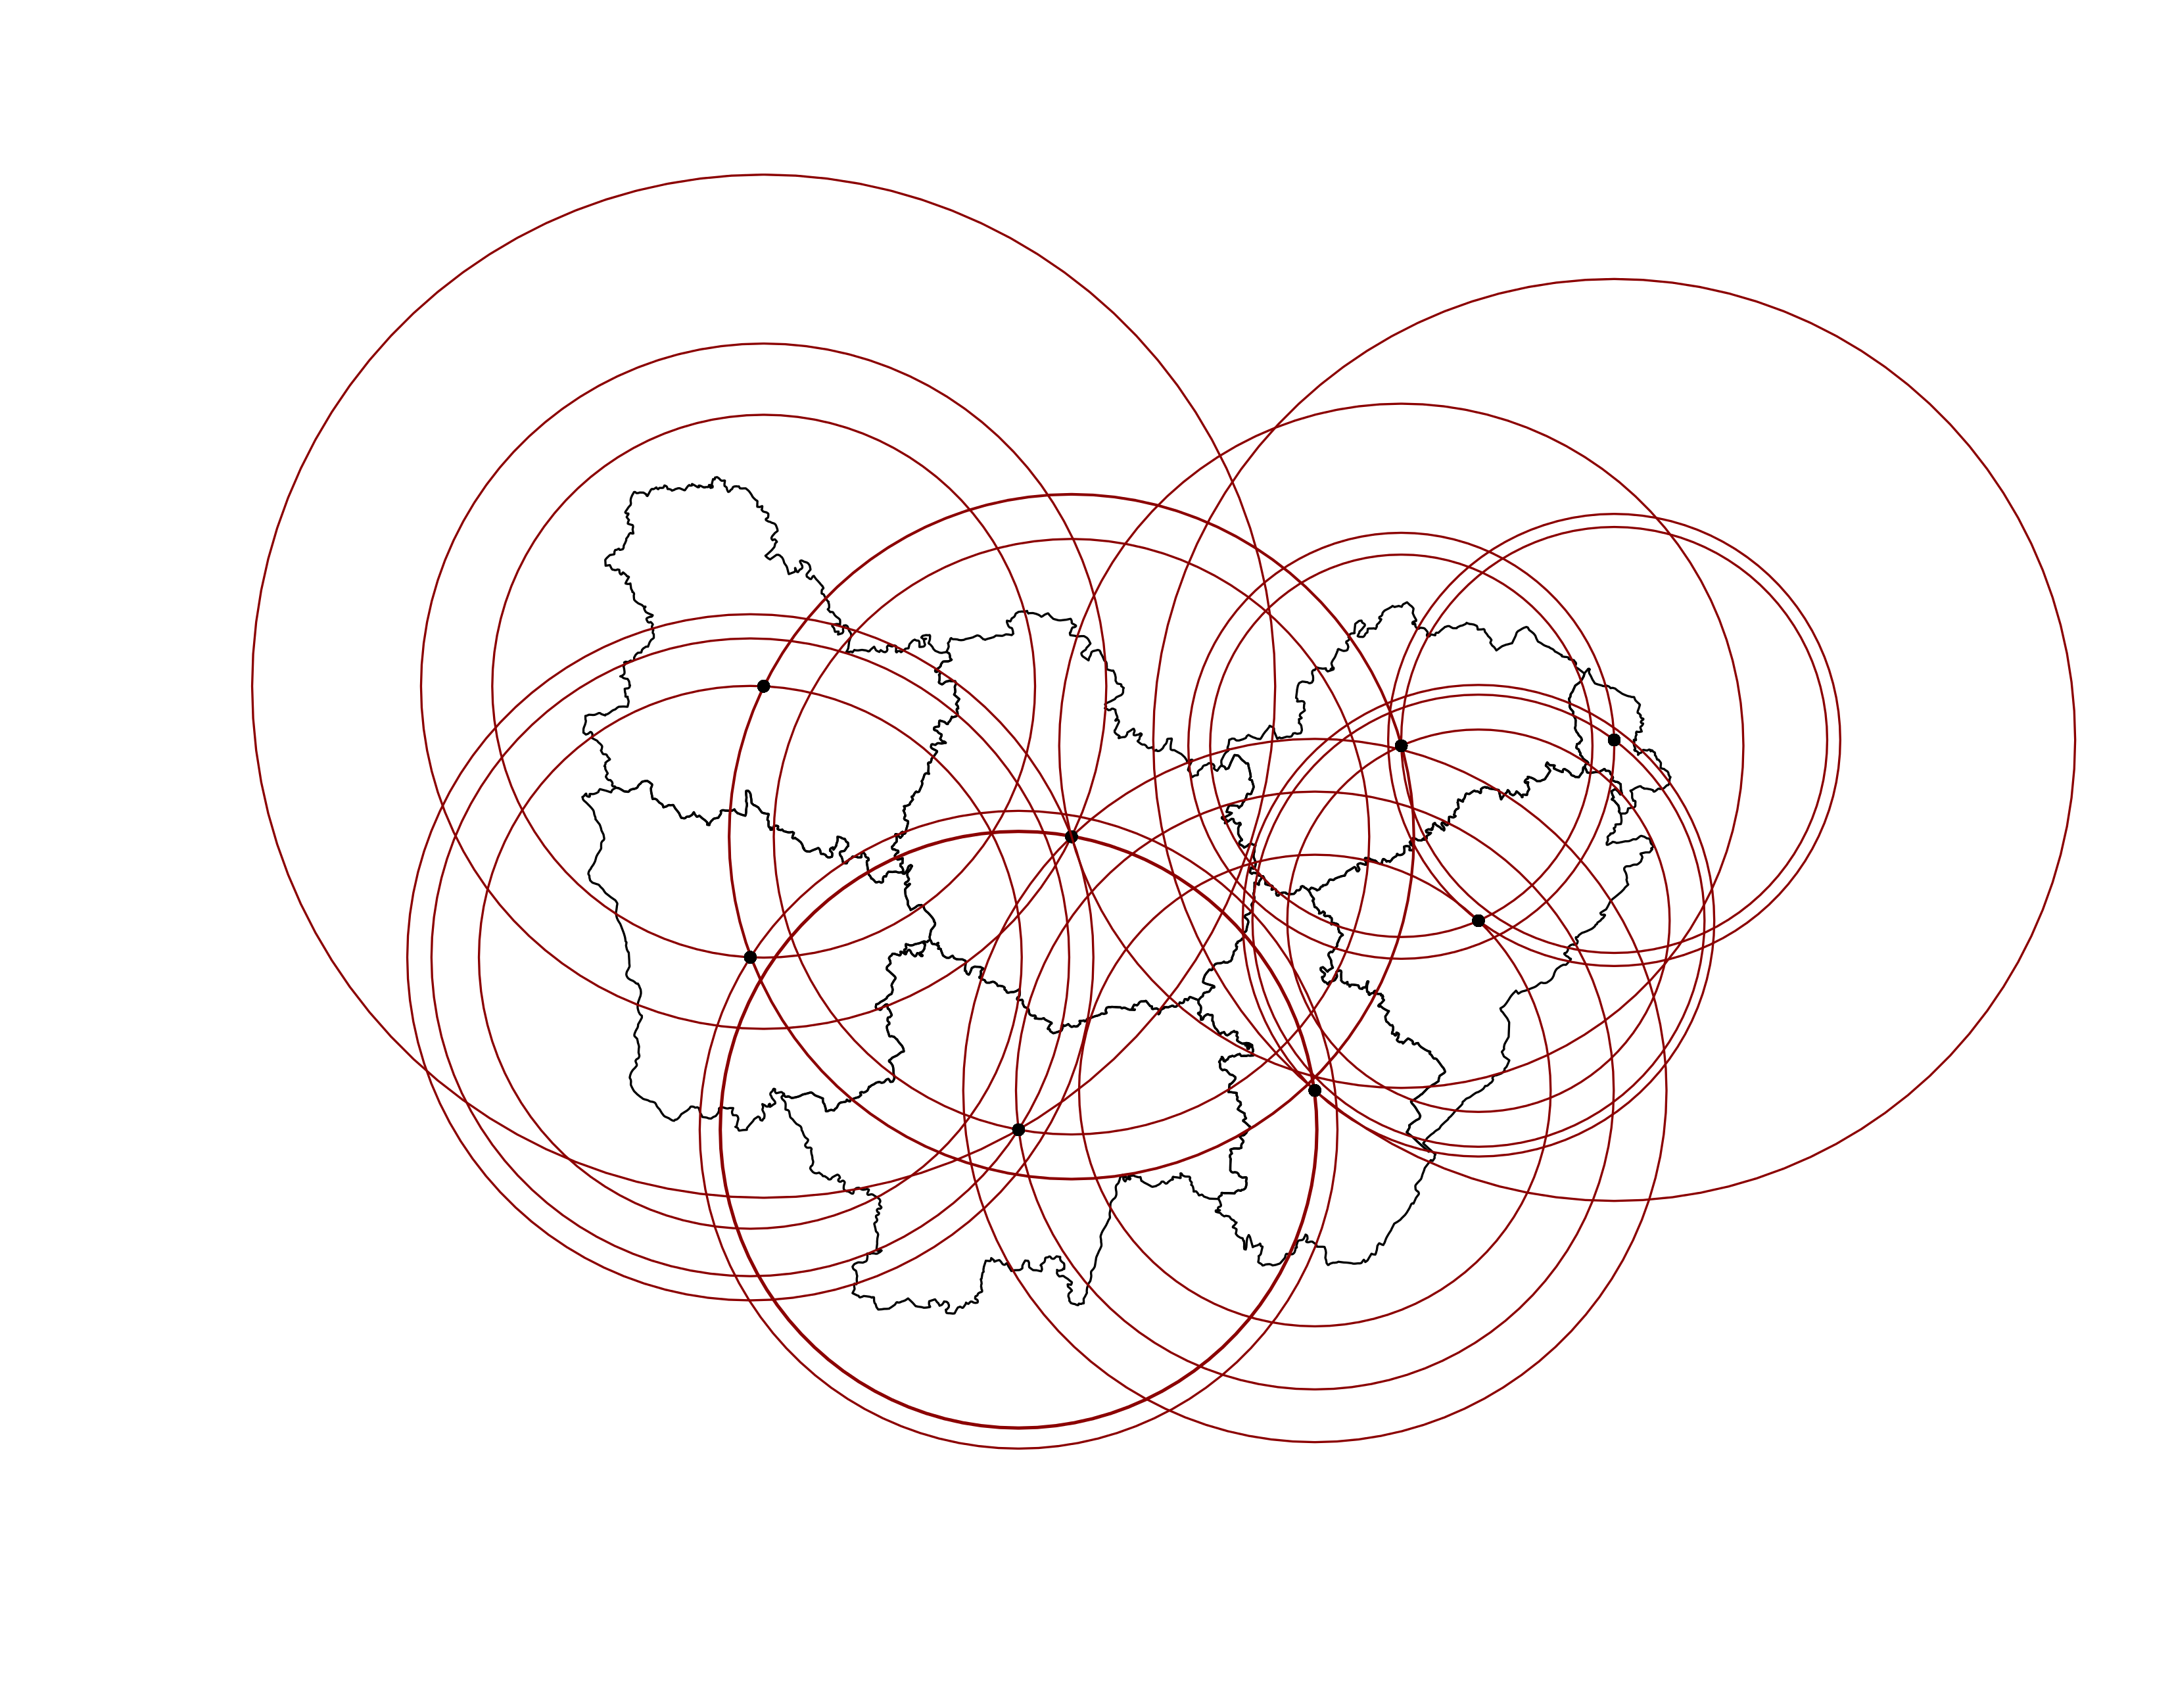
\includegraphics[width=0.6\linewidth]{clusters_all.png}
\caption{Set of potential clusters defined with a circular scanning window of variable center and radius with Equation~\ref{eq:cluster} on a set of eight administrative areas in France. Each potential cluster is represented with a red circle.}
\label{fig:potentialclusters}
\end{figure}

\noindent Then the spatial scan statistic can be defined as the maximum of a concentration index over the set of potential clusters $\mathcal{W}$. The second step is the determination of the statistical significance of the spatial scan statistic. For this, since the distribution of the scan statistic is intractable under $\mathcal{H}_0$ due to the overlapping nature of $\mathcal{W}$, a common approach, which will be considered here, is to use a Monte-Carlo method (see Section~\nameref{sec:signif} for more details).

%For this purpose we use a set of potential clusters $\mathcal{W}$. The approach most often used and introduced by \citet{spatialdisease} is to use circular clusters of variable size. An approach often advised is to limit the maximum size to half of the studied region since otherwise it would be like detecting a ``negative cluster'' in the areas outside the clusters covering almost all the studied region \citep{spatialdisease}. 
% Following the latter's the set of potential clusters is defined by
% \begin{equation} \label{eq:cluster}
% \mathcal{W} = \{ w_{i,j} \ / \ 1 \le |w_{i,j}| \le \frac{n}{2}, \ 1 \le i,j \le n \},
% \end{equation}
% where $w_{i,j}$ is the disc centered on $s_i$ that passes through $s_j$ and $|w_{i,j}|$ corresponds to the number of sites in $w_{i,j}$. 


\subsection{Spatial scan statistics for multivariate data} \label{subsec:multi}

%\textbf{\textit{In a few words.}}
Here we consider the case where several continuous variables are simultaneously observed in each spatial location: $X = (X^{(1)}, \dots, X^{(p)})^\top$ is a $p$-dimensional variable ($p \ge 2$). In this context the objective is to identify multivariate spatial clusters that are aggregations of sites in which $X$ takes higher or lower values (in terms of mean, median, etc.) than elsewhere. For example one could observe the average concentrations of several pollutants over a day: a vector can be associated with each site, each element of which corresponds to the average concentration of one pollutant. In this context a spatial cluster corresponds to a set of sites under or overexposed to multiple pollutants. Different approaches will be presented: a parametric method based on a Gaussian model and a nonparametric one. \\ %On Gaussian data both approaches offer high power and high true positive rates. On the other hand, in the case of non-normal data, the non-parametric method has to be preferred.
Figure~\ref{fig:schema_multi} summarizes the different types of multivariate data with examples, and provides guidelines on the spatial scan statistics methods to be used for these data (and the argument to use in the scan function of the package). More precisely, we distinguish three types of spatial data: lattice data which are aggregated data for example at the scale of the regions of a country, geostatistical data which are defined on a continuous space (typically temperature, sunshine, or atmospheric pressure) although they are observed only at discrete sites, and marked point data for which the location is random (for example the distribution of trees in a forest) and we observe at each location the circumference and height of the tree for example. To detect spatial clusters, in the case of Gaussian data we will prefer the Gaussian approach (MG) and otherwise we will use the nonparametric approach (MNP).\\

\begin{figure}[h!]
\centering
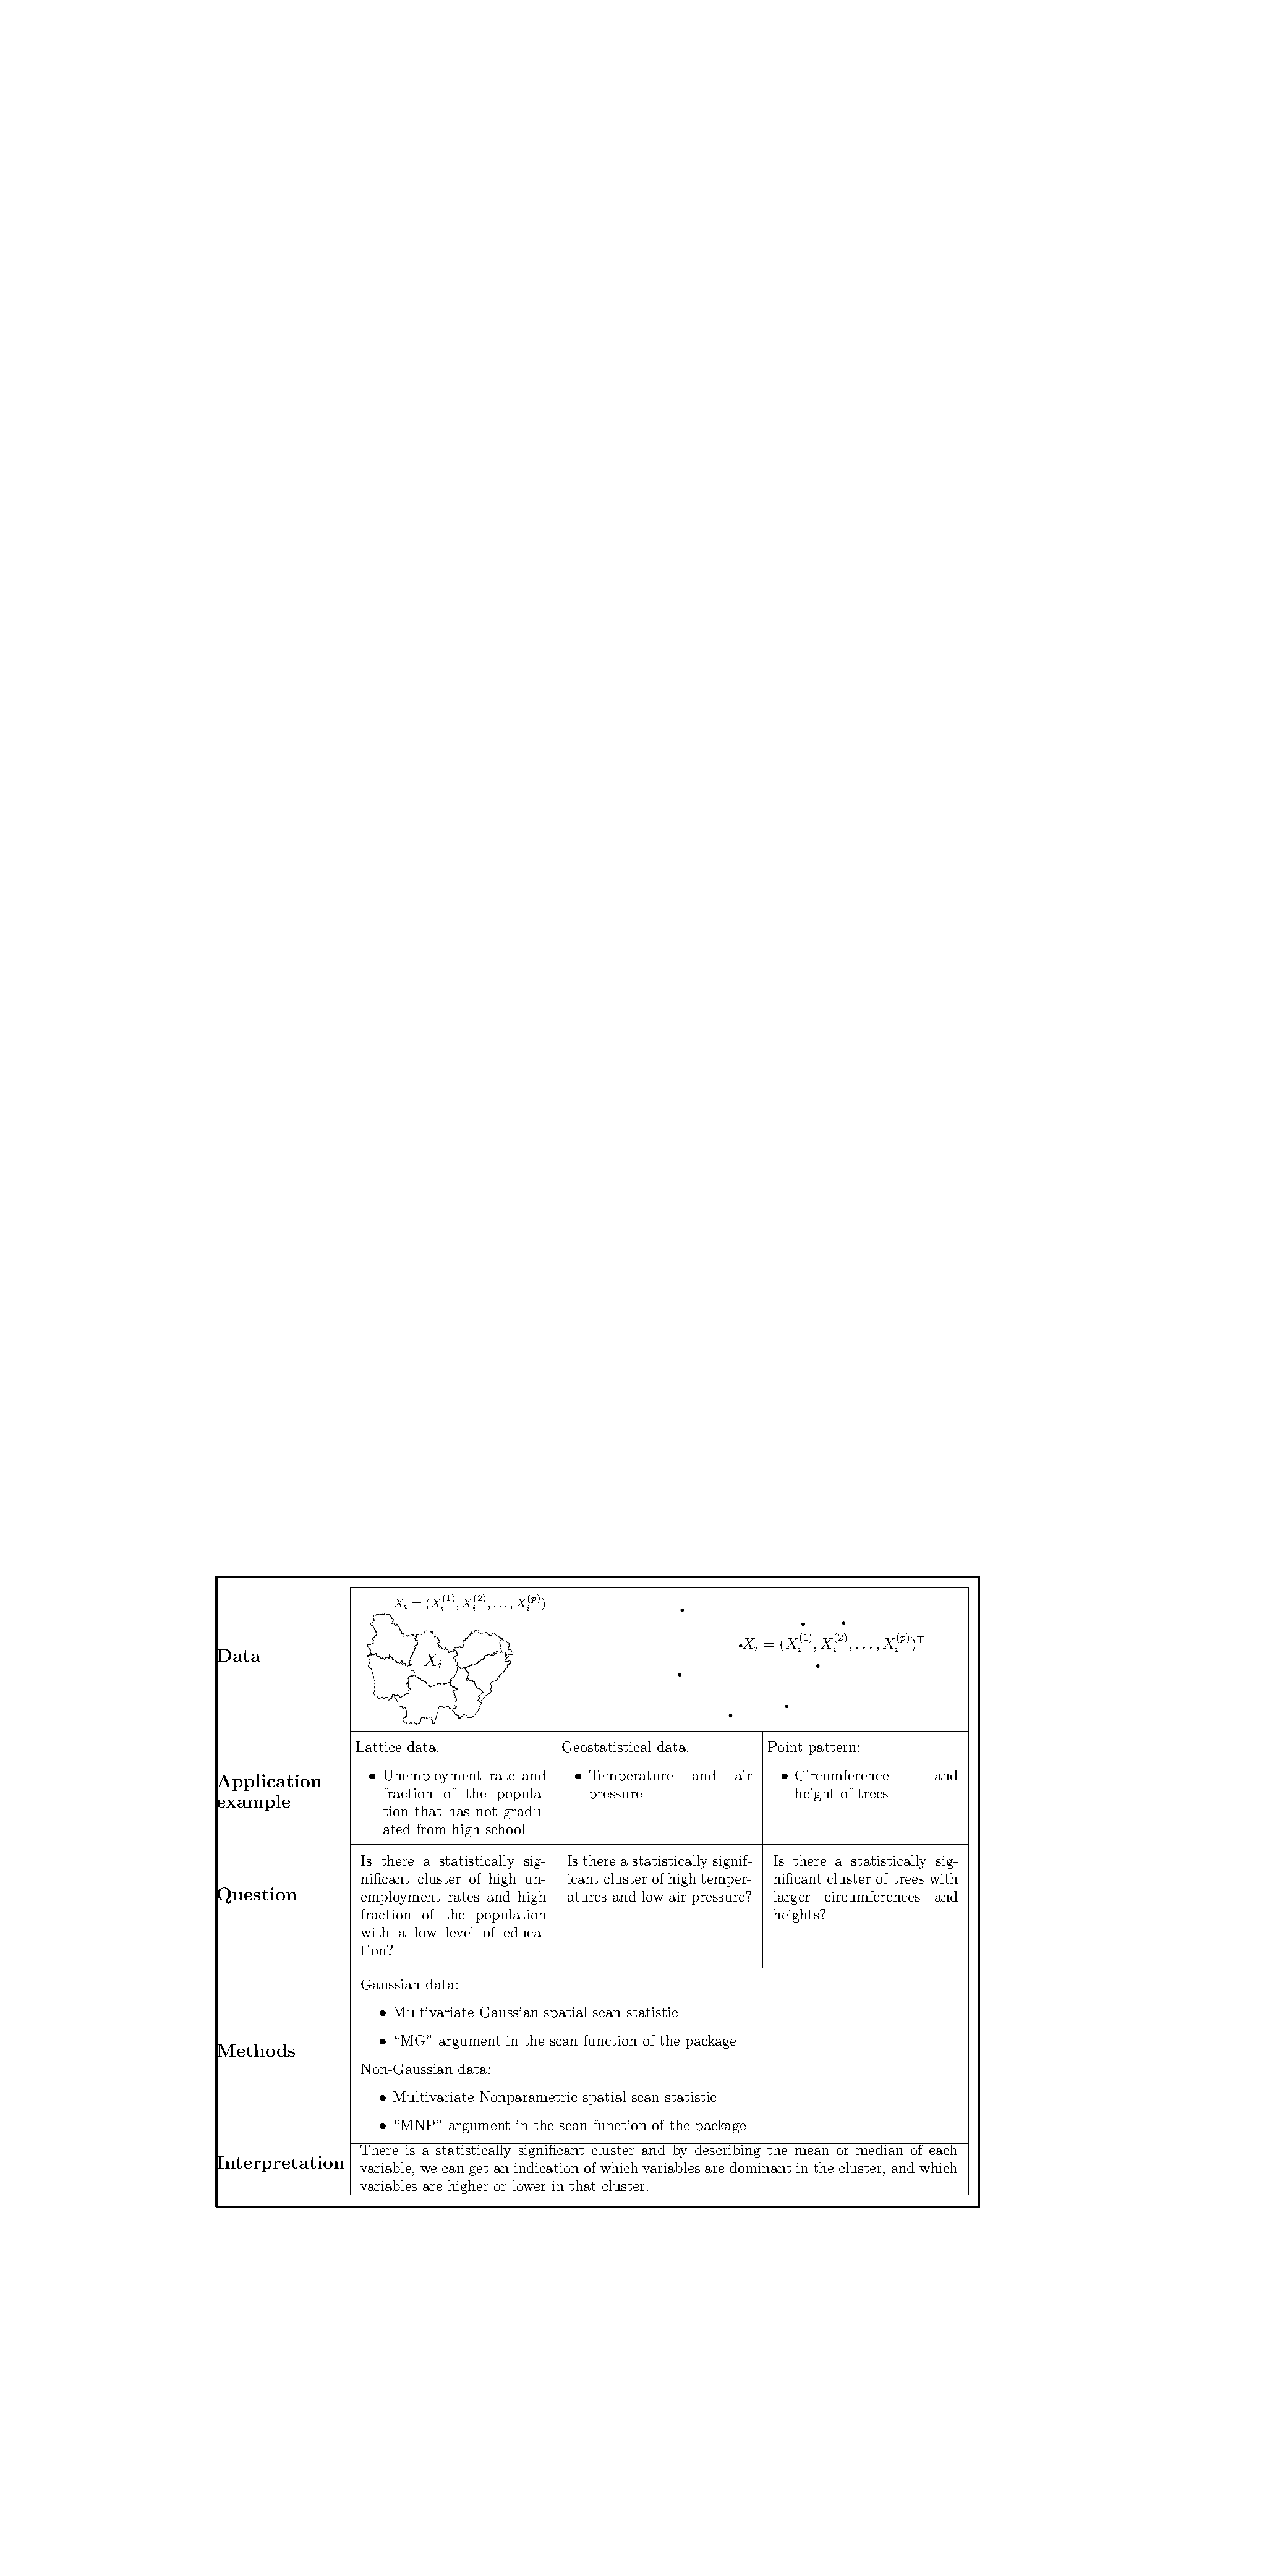
\includegraphics[width=\linewidth]{code_RJ_multi.pdf}
\caption{Summary of spatial scan statistics for multivariate data. The table indicates the question that can be asked for the detection of clusters. It then indicates the methods to be used according to the distribution of the data as well as the ways to interpret the detected clusters.
Spatial scan statistics for multivariate data can be used to detect spatial clusters on any type of spatial data (lattice, geostatistical, point data) modeled by vectors. The detected clusters can be characterized by computing the mean or median of each variable inside and outside each cluster.
% In this figure the data is composed of multivariate vectors $X_i$. Several applications are proposed for lattice, geostatistical, and point data. 
%Summary of the different types of multivariate data and methods of spatial scan statistics for these data
}
\label{fig:schema_multi}
\end{figure}


\noindent \citet{a_multivariate_gaussian} proposed a parametric spatial scan statistic for multivariate data based on a multivariate normal model taking into account the correlations between the variables. \\
The null hypothesis $\mathcal{H}_0$, corresponding to the absence of any cluster in the data, is the
following: $\forall i \in \llbracket 1 ; n \rrbracket, \ X_i \sim \mathcal{N}_p(\mu, \Sigma)$ and the alternative hypothesis $\mathcal{H}_1^{(w)}$
associated with a potential cluster $w$ can be defined as: $\forall i \in \llbracket 1 ; n \rrbracket, \ X_i \sim \left\{ \begin{array}{ll}
\mathcal{N}_p(\mu_w, \Sigma_{w,w^\mathsf{c}}) & \text{ if } s_i \in w \\
\mathcal{N}_p(\mu_{w^\mathsf{c}}, \Sigma_{w,w^\mathsf{c}}) & \text{ otherwise}
\end{array} \right.$. \\

\noindent Then we can compute the MLE estimates of $\mu, \mu_w, \mu_{w^\mathsf{c}}, \Sigma$ and $\Sigma_{w,w^\mathsf{c}}$: $\hat{\mu}, \widehat{\mu}_w, \widehat{\mu}_{w^\mathsf{c}}, \widehat{\Sigma}$ and $\widehat{\Sigma}_{w,w^\mathsf{c}}$, and we can show that the log-likelihood ratio between these two hypotheses is
\begin{align*}
\widehat{LLR^w} = &-\frac{n}{2}\ln\bigg[\text{det}\Big(\sum_{\substack{i\\ s_i \in w}} \left(X_i - \widehat{\mu}_w \right) \left(X_i - \widehat{\mu}_w \right)^\top + \sum_{\substack{i \\ s_i \in w^\mathsf{c}}} \left(X_i - \widehat{\mu}_{w^\mathsf{c}} \right) \left(X_i - \widehat{\mu}_{w^\mathsf{c}} \right)^\top \Big)\bigg] \\
&+ \frac{n}{2}\ln\bigg[\text{det}\Big(\sum_{i=1}^{n} \left(X_i - \hat{\mu} \right) \left(X_i - \hat{\mu} \right)^\top \Big)\bigg],  
\end{align*}
where $\displaystyle{ \hat{\mu}_g = \dfrac{1}{|g|} \sum_{i, s_i \in g} X_i }$ for $g \in \{ w, w^\mathsf{c} \}$ and $ \displaystyle{  \hat{\mu} = \dfrac{1}{n} \sum_{i=1}^n X_i } $. \\

\noindent Finally the log-likelihood ratio is used as a concentration index and maximised over the set of potential clusters $\mathcal{W}$. \\ Thus we can show that the multivariate Gaussian (MG) scan statistic is $$\lambda_{\text{MG}} = \underset{w \in \mathcal{W}}{\min} \ \text{det}\Big(\sum_{\substack{i\\ s_i \in w}} \left(X_i - \widehat{\mu}_w \right) \left(X_i - \widehat{\mu}_w \right)^\top + \sum_{\substack{i \\ s_i \in w^\mathsf{c}}} \left(X_i - \widehat{\mu}_{w^\mathsf{c}} \right) \left(X_i - \widehat{\mu}_{w^\mathsf{c}} \right)^\top \Big).$$

\noindent This test performs very
well against Gaussian alternatives but faces problems when the data is
not normal, which is often the case when dealing with environmental data
exhibiting extreme values. For that reason \citet{nonparam_multi} developed a nonparametric spatial scan statistic for multivariate data based on a multivariate extension of the Wilcoxon-Mann-Whitney test for multivariate data \citep{oja}. \\
In this context the null hypothesis $\mathcal{H}_0$ can be rewritten as $\mathcal{H}_0: X_1, \dots, X_n$ are identically distributed, whatever the associated location. \\
Let $$\begin{array}{ccccl}
\text{sgn} & : & \mathbb{R}^p & \to & \mathbb{R}^p \\
 & & x & \mapsto & \left\{
\begin{array}{cl}
  ||x||_2^{-1} x & \text{ if } x \neq 0 \\
  0 & \text{ otherwise}
\end{array}
\right. \\
\end{array},$$ then the multivariate ranks $R_i$ are defined by $\displaystyle{R_i = \dfrac{1}{n} \sum_{j=1}^{n} \text{sgn}(A_X(X_i - X_j))}$ where the matrix $A_X$ makes the ranks such that $\displaystyle{\dfrac{p}{n}\sum_{i=1}^{n} R_i R_i^\top = \dfrac{1}{n} \sum_{i=1}^{n} R_i^\top R_i I_p}$. Note that this matrix can be easily computed using an iterative procedure.
Then the multivariate
extension of the Wilcoxon-Mann-Whitney statistic proposed by \citet{oja} is $$U^2(w) = \dfrac{p}{c^2_X} \left[\ |w| \ ||\bar{R}_w||_2^2 + |w^\mathsf{c}| \ ||\bar{R}_{w^\mathsf{c}}||_2^2 \ \right], \text{ where } \displaystyle{c^2_X = \dfrac{1}{n}\sum_{i=1}^n R_i^\top R_i}. $$

\noindent \citet{nonparam_multi} used $U^2(w)$ as a concentration index to build the spatial scan statistic: the multivariate nonparametric (MNP) scan
statistic is $\lambda_{\text{MNP}} = \underset{w \in \mathcal{W}}{\max} \ U^2(w)$.

\noindent It should be noted that in the case $p=1$, these statistics are respectively equivalent  to the ones introduced by \citet{normalkulldorff} (which is equivalent to the scan statistic developed by \citet{a_distribution_free}, UG), and \citet{A_nonparametric_spatial} (UNP).

\subsection{Spatial scan statistics for univariate functional data}

%\textbf{\textit{In a few words.}}
Here we consider the case where a continuous variable is observed in each spatial location over time: $\{ X(t), \ t \in \mathcal{T} \}$ is a real-valued stochastic process where $\mathcal{T}$ is an interval of $\mathbb{R}$. In this context the objective is to identify functional spatial clusters that are aggregations of sites in which the curves are higher or lower than elsewhere. For example, one can observe the concentration of an air pollutant over time in different geographical areas. Then a cluster corresponds to an aggregation of sites in which the concentration of the air pollutant is higher or lower over the time than in the other spatial units. Several methods will be considered: a parametric method based on a functional ANOVA, a nonparametric approach using a Wilcoxon-Mann-Whitney test for high-dimensional data, a distribution-free approach based on a pointwise Student's t-test and finally a pointwise rank-based method. On Gaussian data, for non localized clusters in time all approaches show high power and high true positive rates. However the performances of the ANOVA-based method strongly decrease on non-normal data. For localized clusters in time (that are aggregations of sites that take higher or lower values for $X$ only in a small interval of time (an interval of five days over a study period of one month for example)) the pointwise approaches should be favored. \\
Figure~\ref{fig:schema_unifonc} summarizes the different types of univariate functional data with examples, and provides recommendations on the spatial scan statistics methods to be used for these data (and the argument to use in the scan function of the package). More precisely, we distinguish lattice functional data which are aggregated functional data for example at the scale of the administrative areas of a country (unemployment rate, percentage of the population over 65, etc), geostatistical functional data which are defined on a continuous space (typically temperature, sunshine, or atmospheric pressure over time) although they are observed only at discrete sites, and marked point data for which the location is random (for example the distribution of trees in a forest) and we observe at each location the circumference of the tree over time for example. To detect spatial clusters, as mentioned before, in the case of Gaussian data we will prefer the pointwise distribution-free functional approach (DFFSS) and otherwise we will use the pointwise rank-based approach (URBFSS). \\

\begin{figure}[h!]
\centering
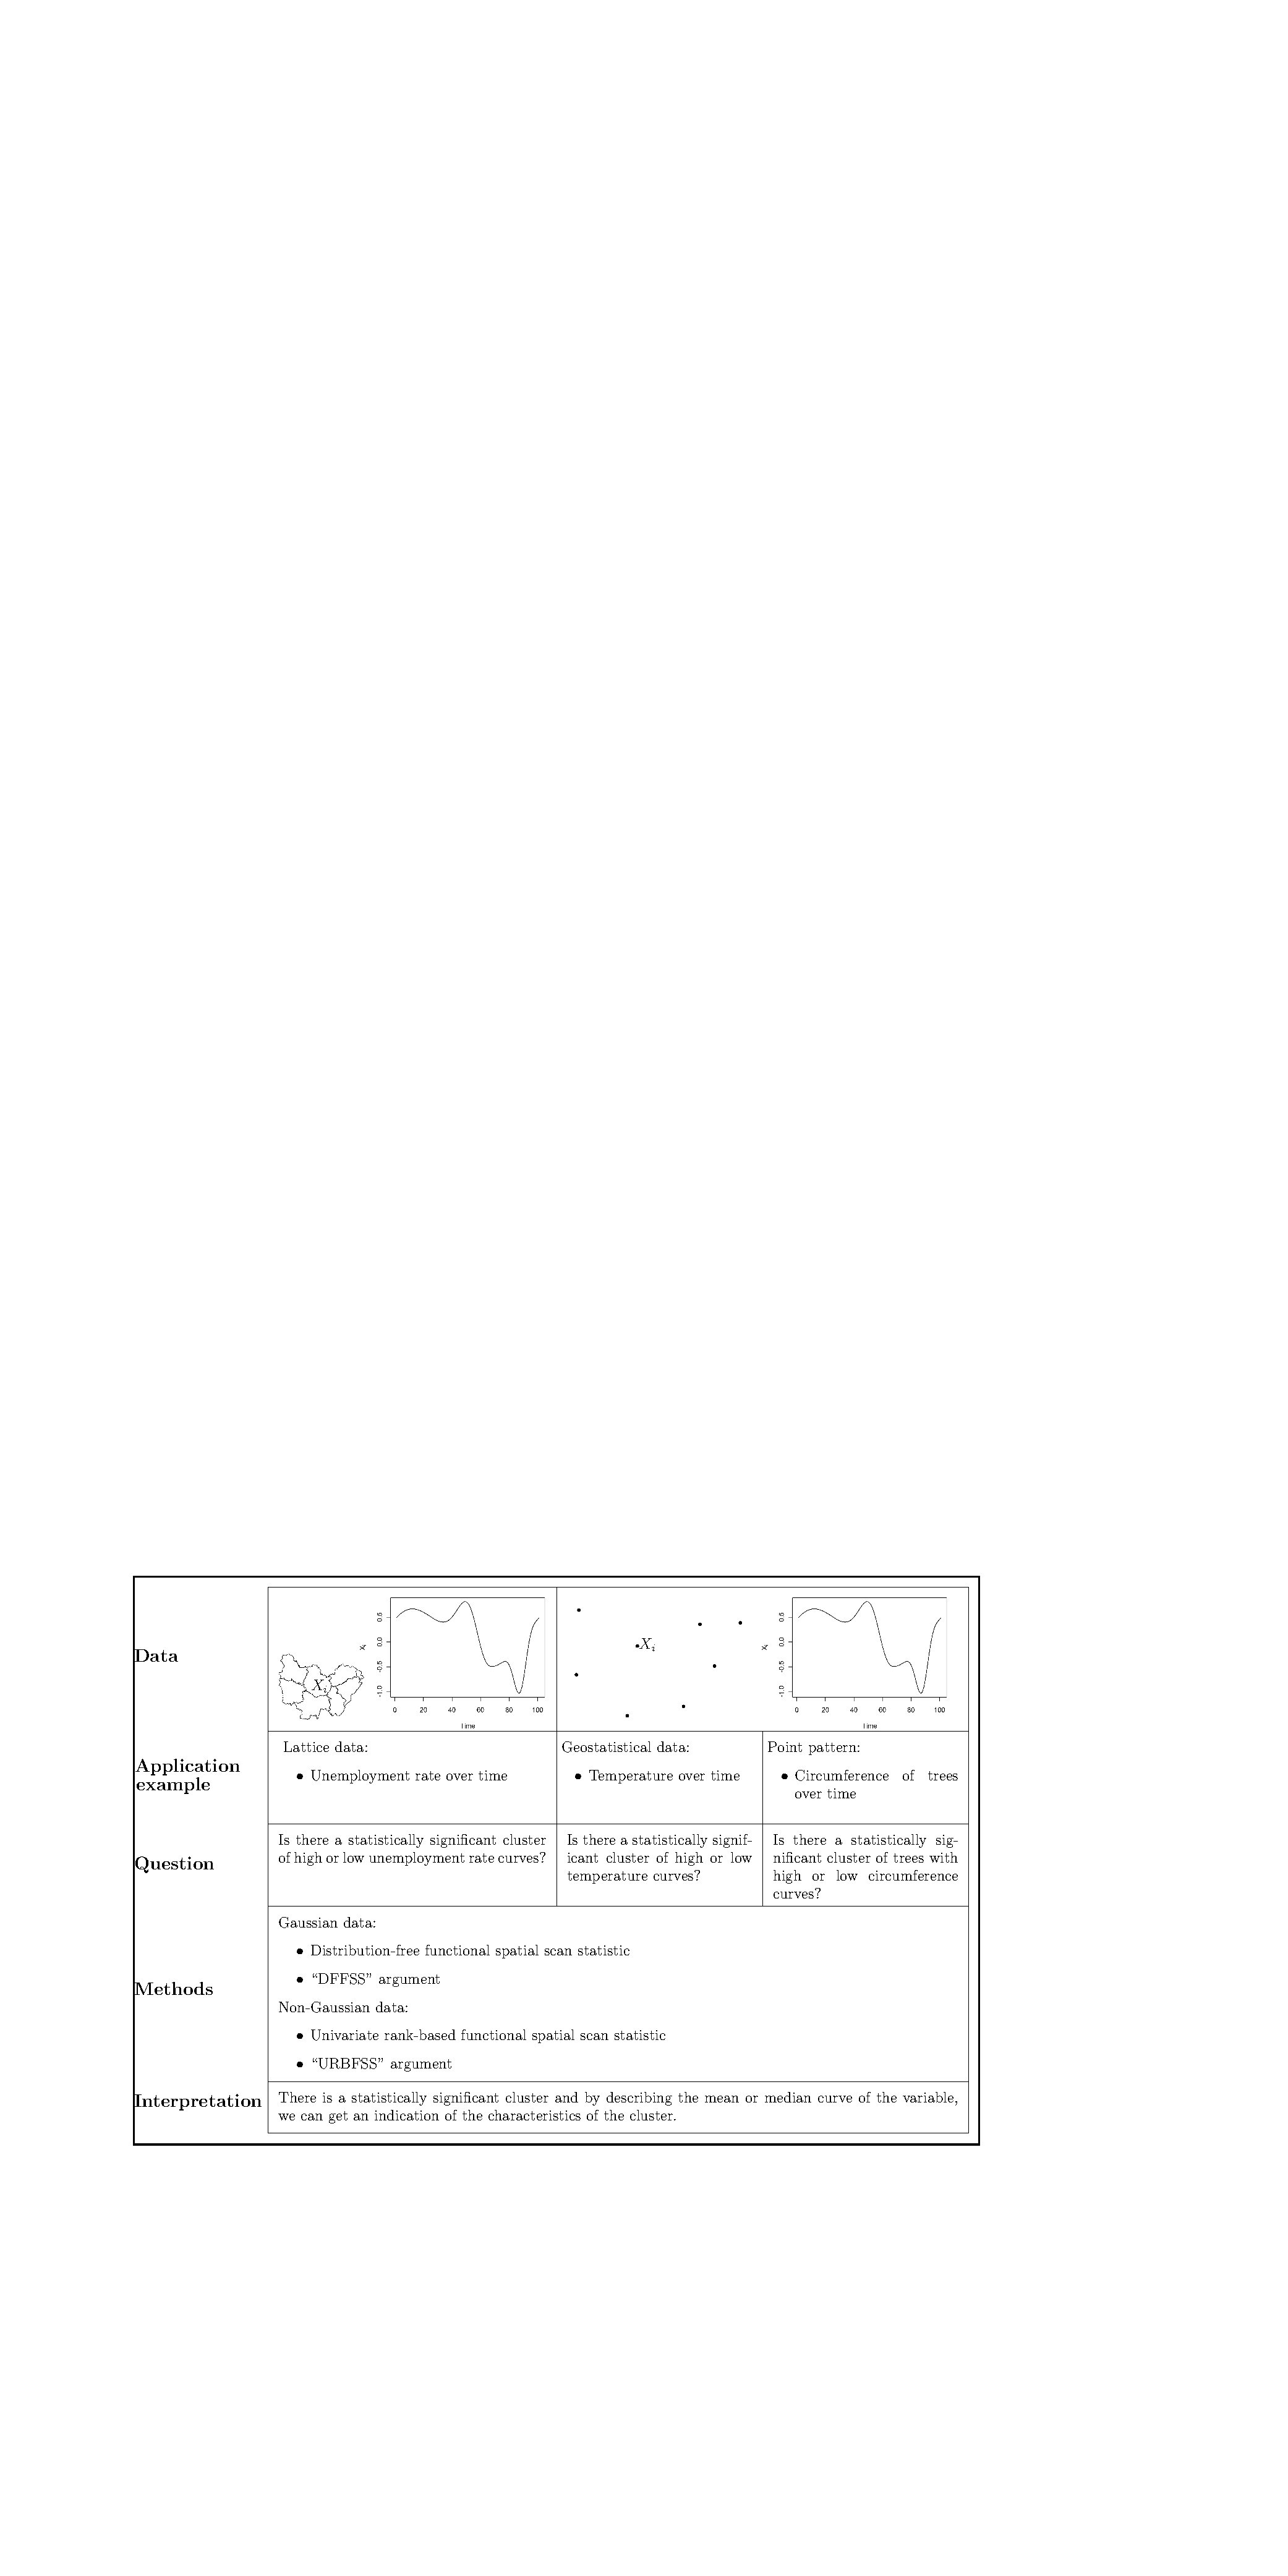
\includegraphics[width=\linewidth]{code_RJ_unifonc.pdf}
\caption{Summary of spatial scan statistics for univariate functional data. The table indicates the question that can be asked for the detection of clusters on a set of curves. It then indicates the methods to be used according to the distribution of the data as well as the ways to interpret the detected clusters.
Spatial scan statistics for univariate functional data can be used to detect spatial clusters on any type of spatial data (lattice, geostatistical, point data) observed over a period of time. The detected clusters can be characterized by computing the mean or median curve inside and outside each cluster.
% In this figure the data is a set of curves $X_i$. Several applications are proposed for lattice, geostatistical, and point data. For each of these data,  %\textcolor{red}{Spatial scan statistics for univariate functional data allow the detection of spatial clusters of univariate spatial processes (lattice, geostatistical or marked point processes) observed over time.}
%Summary of the different types of univariate functional data and methods of spatial scan statistics for these data
}
\label{fig:schema_unifonc}
\end{figure}

\subsubsection{The parametric spatial scan statistic for univariate functional data}

\noindent \citet{notre_fonctionnel} supposed that the process $X$ takes values in a semi-metric space, in particular in $\mathcal{L}^2(\mathcal{T},\mathbb{R})$ and proposed a parametric spatial scan statistic for functional data, based on a functional ANOVA. Here the null hypothesis $\mathcal{H}_0$ can be rewritten: $\mathcal{H}_0: \forall w \in \mathcal{W}, \ \mu_{w} = \mu_{w^\mathsf{c}} = \mu_S$, and the alternative hypothesis $\mathcal{H}_1^{(w)}$ associated with a potential cluster $w$ can be defined as follows: $\mathcal{H}_1^{(w)}: \mu_{w} \neq \mu_{w^\mathsf{c}}$, where $\mu_w$, $\mu_{w^\mathsf{c}}$ and $\mu_S$ stand for the mean functions in $w$, outside $w$ and over $S$, respectively. \citet{anova_functional} and \citet{comparisonanova} proposed the following ANOVA test statistic:
$$
\displaystyle{F_n^{(w)} = \dfrac{
|w| \ ||\bar{X}_{w} - \bar{X}||_2^2 + |w^\mathsf{c}|  \  ||\bar{X}_{w^\mathsf{c}} - \bar{X}||_2^2}{ \dfrac{1}{n-2}
\left[\sum_{j, s_j \in w} ||X_j - \bar{X}_{w}||_2^2 + \sum_{j, s_j \in w^\mathsf{c}} ||X_j - \bar{X}_{w^\mathsf{c}}||_2^2 \right]},}
$$
where $\displaystyle{\bar{X}_{g}(t) = \dfrac{1}{|g|} \sum_{i, s_i \in g} X_i(t)}$ are empirical estimators of $\mu_g$ ($g \in \{w, w^\mathsf{c}\}$), $\displaystyle{\bar{X}(t) = \dfrac{1}{n} \sum_{i = 1}^n X_i(t)}$ is the empirical estimator of $\mu_S$ and $\displaystyle{||x||_2^2 = \int_{\mathcal{T}} x^2(t) \ \text{d}t}$. \\

\noindent Thus, \citet{notre_fonctionnel} proposed to use $F_n^{(w)}$ as a concentration index and the proposed parametric functional spatial scan statistic (PFSS) is $\Lambda_{\text{PFSS}} = \underset{w \in \mathcal{W}}{\max} \  F_n^{(w)}$. \\

\noindent This method gives high powers and F-measures on normal data but as in the multivariate framework the parametric method faces problems when the data is not normal. \citet{wilco_cucala} proposed a nonparametric spatial scan statistic for functional data based on a functional Wilcoxon-Mann-Whitney test \citep{wilco}. \\

\subsubsection{A nonparametric spatial scan statistic for functional data}


\noindent Here $X$ is a process of a smooth Banach space $\chi$, with a  Gâteaux differentiable norm $||.||_{\chi}$. Let denote $P_w$ and $P_{w^\mathsf{c}}$ the probability measures of $X$ in $w$ and in $w^\mathsf{c}$ respectively, then $\mathcal{H}_0$ corresponds to: $\mathcal{H}_0: \forall w \in \mathcal{W}, \ P_w = P_{w^\mathsf{c}}$ and the alternative hypothesis associated with a potential cluster $w$ can be rewritten as $\mathcal{H}_1^{(w)}: P_w(X) = P_{w^\mathsf{c}}(X-\Delta), \ \Delta \in \chi \backslash \{0\}$. \\
\citet{wilco} defined the sign function in the functional framework as 
$$\forall h \in \chi, \ \text{Sgn}_X(h) = \left\{ \begin{array}{cl} \underset{v \rightarrow 0^+}{\lim} \ \dfrac{|| X + vh ||_\chi - ||X||_\chi}{v} &\text{ if } X \neq 0 \\
0 &\text{ if } X = 0 \end{array} \right. .$$
Then they proposed the following test statistic:
$$T_{WMW}(w) = \dfrac{1}{|w| |w^\mathsf{c}|} \sum_{i, s_i \in w} \sum_{j, s_j \in w^\mathsf{c}} \text{Sgn}_{X_j - X_i}.$$
Under $\mathcal{H}_0$, if $\dfrac{|w|}{n} \rightarrow \gamma \in [0;1]$ as $|w|, |w^\mathsf{c}| \rightarrow \infty$, $\sqrt{\dfrac{|w| |w^\mathsf{c}|}{n}} T_{WMW}(w)$ converges weakly to a distribution that does not depend on $|w|$. Thus \citet{wilco_cucala} proposed to use $U(w) = \bigg| \bigg| \sqrt{\dfrac{|w| |w^\mathsf{c}|}{n}} T_{WMW}(w) \bigg| \bigg|$ as a concentration index: the nonparametric functional scan statistic (NPFSS) is $\Lambda_{\text{NPFSS}} = \underset{w \in \mathcal{W}}{\max} \ U(w)$. \\ It should be noticed that although \citet{wilco_cucala} only studied the performances of the NPFSS in the univariate functional framework, their method is also applicable on multivariate functional data as shown by \citet{notre_fonctionnel1}.

\subsubsection{A distribution-free spatial scan statistic for univariate functional data}

\citet{notre_fonctionnel} also proposed to combine the distribution-free spatial scan statistic for univariate data proposed by \citet{a_distribution_free} and the max statistic of \citet{hd_manova}. They supposed that for each time $t$, $\mathbb{V}[X_i(t)] = \sigma^2(t)$ for all $i \in \llbracket 1 ; n \rrbracket$. Then for each $t$, the concentration index proposed by \citet{a_distribution_free} to test $\mathcal{H}_0: \forall w \in \mathcal{W}, \mu_w(t) = \mu_{w^\mathsf{c}}(t) = \mu_S(t)$ was 
$$I^{(w)}(t) = \dfrac{|\bar{X}_w(t) - \bar{X}_{w^\mathsf{c}}(t)|}{\sqrt{\hat{\mathbb{V}}[\bar{X}_w(t) - \bar{X}_{w^\mathsf{c}}(t)]}}, $$
where $\hat{\mathbb{V}}[\bar{X}_w(t) - \bar{X}_{w^\mathsf{c}}(t)] = \widehat{\sigma^2}(t) \left[ \dfrac{1}{|w|} + \dfrac{1}{|w^\mathsf{c}|} \right] $, \\ $\displaystyle{\widehat{\sigma^2}(t) = \dfrac{1}{n-2} \left[ \sum_{i, s_i \in w} (X_i(t) - \bar{X}_w(t))^2 + \sum_{i, s_i \in w^\mathsf{c}} (X_i(t) - \bar{X}_{w^\mathsf{c}}(t))^2 \right]}$. \\

\noindent Then the idea is to globalize the information by maximizing the previous quantity over the time for each potential cluster $w$, as suggested by \citet{hd_manova}:
$$ I^{(w)} = \underset{t \in \mathcal{T}}{\sup} \ I^{(w)}(t).$$

\noindent For cluster detection, as for the PFSS, the null hypothesis $\mathcal{H}_0$ (the absence of cluster) is defined as follows: $\mathcal{H}_0: \forall w \in \mathcal{W}, \ \mu_{w} = \mu_{w^\mathsf{c}} = \mu_S$. And the alternative hypothesis $\mathcal{H}_1^{(w)}$ associated with a potential cluster $w$ can be defined as follows: $\mathcal{H}_1^{(w)}: \mu_{w} \neq \mu_{w^\mathsf{c}}$. \\

\noindent \citet{notre_fonctionnel} considered $I^{(w)}$ as a concentration index and maximized it over the set of potential clusters $\mathcal{W}$ yielding to the following distribution-free functional spatial scan statistic (DFFSS): $
\Lambda_{\text{DFFSS}} = \underset{w \in \mathcal{W}}{\max} \  I^{(w)}$.



\subsubsection{A new rank-based spatial scan statistic for univariate functional data}

A pointwise approach based on ranks and on the nonparametric scan statistic for univariate data \citep{A_nonparametric_spatial} can be proposed in the univariate functional framework by adapting the approach of \citet{notre_fonctionnel1}.

\noindent For a time $t$, \citet{A_nonparametric_spatial} proposed to test $\mathcal{H}_0: \forall w \in \mathcal{W}, F_{w,t} = F_{w^\mathsf{c},t}$ where $F_{w,t}$ and $F_{w^\mathsf{c},t}$ are the cumulative distribution functions of $X(t)$ in $w$ and outside $w$, by using the
Wilcoxon rank-sum test statistic. For a time $t$ and a potential cluster $w$, the Wilcoxon rank-sum test statistic is $\displaystyle{W(t)^{(w)} = \sum_{i, s_i \in w} R_i(t)}$ where $R_i(t)$ is the rank of $X_i(t)$ in $\{ X_1(t), \dots, X_n(t) \}$, using the average rank in the case of tied observations. \\
Then the standardized version of this statistic is $$T(t)^{(w)} = \dfrac{W(t)^{(w)} - \mathbb{E}[W(t)^{(w)}]}{\sqrt{\mathbb{V}[W(t)^{(w)}]}}$$ where 
$\mathbb{E}[W(t)^{(w)}] = \dfrac{|w|(n+1)}{2}$ and $\mathbb{V}[W(t)^{(w)}] = \dfrac{|w| |w^\mathsf{c}| (n+1)}{12}$ are the expected value and the variance of $W(t)^{(w)}$ under $\mathcal{H}_0$. \\ \citet{A_nonparametric_spatial} proposed to minimize the p-value associated with $T(t)^{(w)}$ on the set of potential clusters $\mathcal{W}$. We propose to adapt their approach by simply using $|T(t)^{(w)}|$ as a pointwise statistic. \\

\noindent In the context of cluster detection, the null hypothesis is defined as $\mathcal{H}_0$: $\forall w \in \mathcal{W}, \ \forall t \in \mathcal{T}, \ F_{w,t} = F_{w^\mathsf{c},t}$. The alternative hypothesis $\mathcal{H}_1^{(w)}$ associated with a potential cluster $w$ is $\mathcal{H}_1^{(w)}$: $\exists t \in \mathcal{T}, \ F_{w,t}(x) = F_{w^\mathsf{c},t}(x-\Delta_t)$, $\Delta_t \neq 0$. \\

\noindent As before, we propose to globalize the information over the time with $T^{(w)} = \underset{t \in \mathcal{T}}{\sup} \ |T(t)^{(w)}|$ and to use this quantity as a concentration index, yielding to the following univariate rank-based functional spatial scan statistic (URBFSS): $\Lambda_{\text{URBFSS}} = \underset{w \in \mathcal{W}}{\max} \ T^{(w)}$.


\subsection{Spatial scan statistics for multivariate functional data}

%\textbf{\textit{In a few words.}}
Here we consider the case where several continuous variables are observed simultaneously in each spatial unit over time: $\{ X(t), \ t \in \mathcal{T} \}$ is a $p$-dimensional vector-valued stochastic process ($p \ge 2$) where $\mathcal{T}$ is an interval of $\mathbb{R}$. The objective is to detect multivariate functional spatial clusters that are aggregations of sites in which the curves are higher or lower than elsewhere. 
For example we can observe the concentration of several pollutants over time in different locations. Thus at each location we observe several processes (air pollutant concentrations) and these processes can be correlated.
In this context a cluster is an aggregation of sites overexposed or underexposed to multiple pollutants over time. Several methods will be presented: a parametric method based on a functional MANOVA, a distribution-free approach based on a pointwise Hotelling $T^2$-test and finally a pointwise rank-based method. On normal data, all approaches show high power and high true positive rates for non localized clusters in time. However the performances of the methods based on the MANOVA and the Hotelling $T^2$-test decrease on non-normal data. For localized clusters in time the pointwise approaches should be favored, especially the pointwise rank-based method on non-Gaussian data. By localized clusters in time we mean aggregations of sites that take higher or lower values for $X$ only in a small interval of time (an interval of five days over a study period of one month for example). \\
Figure~\ref{fig:schema_multifonc} summarizes the different types of multivariate functional data with examples, and provides guidelines on the spatial scan statistics methods to be used for these data (and the argument to use in the scan function of the package). To be more precise, we can distinguish lattice functional data which are aggregated data for example at the scale of the regions of a country (unemployment rate and fraction of the population that has not graduated from high school, over time, for example), geostatistical functional data which are defined on a continuous space (temperature, sunshine, and atmospheric pressure over time) although they are observed only at discrete sites, and marked point data for which the location is random (for example the distribution of trees in a forest) and we observe at each location the circumference and height of the tree over time for example. As previously mentioned, to detect spatial clusters, in the case of Gaussian data we will prefer the multivariate distribution-free functional spatial scan statistic (MDFFSS) and for non-Gaussian data we will use the pointwise rank-based approach (MRBFSS).\\

\begin{figure}[h!]
\centering
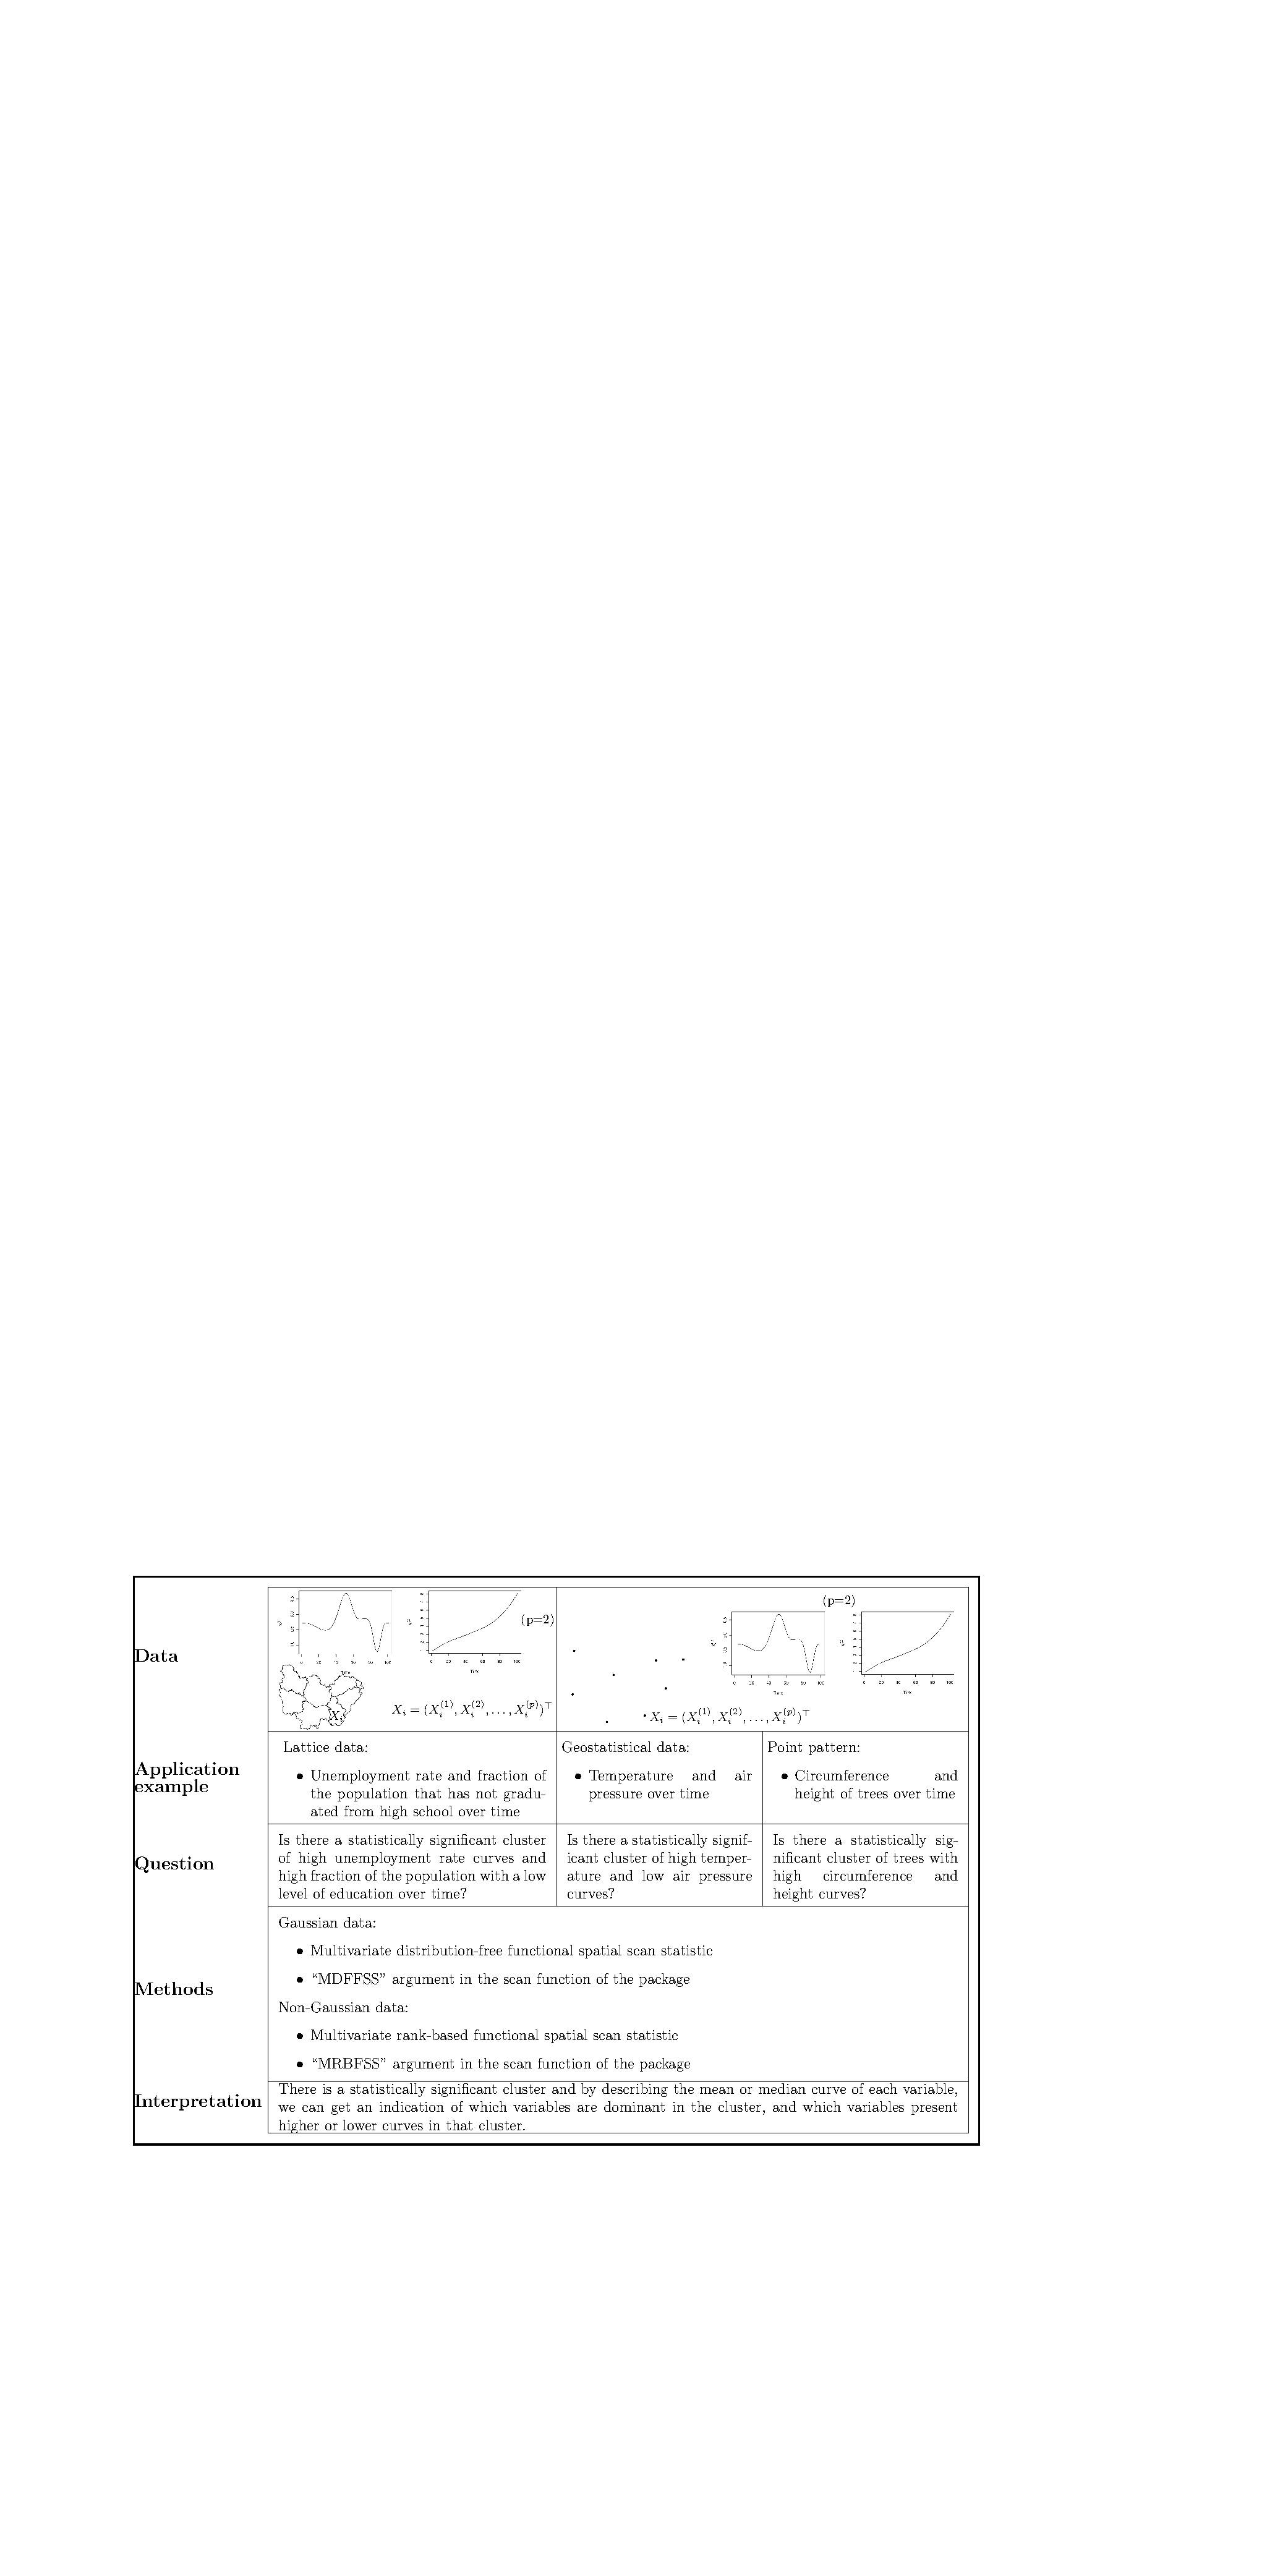
\includegraphics[width=\linewidth]{code_RJ_multifonc.pdf}
\caption{Summary of spatial scan statistics for multivariate functional data. The table indicates the question that can be asked for the detection of clusters of multivariate curves. It then indicates the methods to be used according to the distribution of the data as well as the ways to interpret the detected clusters.
Spatial scan statistics for multivariate functional data can be used to detect spatial clusters on any type of spatial data (lattice, geostatistical, point data) composed of multivariate curves $X_i$ (in the table example, $X_i = (X_i^{(1)}, X_i^{(2)})^\top$ is composed of two curves). Then, the detected clusters can be characterized by computing the mean or median curve of each variable inside and outside each cluster.
% In this figure the data is a set of . Examples of applications are proposed for lattice, geostatistical, and point data. For each of these data,  
%Summary of the different types of multivariate functional data and methods of spatial scan statistics for these data
}
\label{fig:schema_multifonc}
\end{figure}


\subsubsection{A parametric spatial scan statistic for multivariate functional data}


\noindent Here, the process $X$ is supposed to take values in a semi-metric space, in particular the Hilbert space $\mathcal{L}^2(\mathcal{T}, \mathbb{R}^p)$ of $p$-dimensional vector-valued square-integrable functions on $\mathcal{T}$, equipped with the inner product $\displaystyle{\langle X, Y \rangle = \int_{\mathcal{T}} X(t)^\top Y(t) \ \text{d}t}$.

\noindent \citet{notre_fonctionnel1} proposed a parametric scan statistic for multivariate functional data based on a functional MANOVA Lawley–Hotelling trace test \citep{manovafonctional}.  \\

\noindent In this context, the null hypothesis $\mathcal{H}_0$ is $\mathcal{H}_0: \forall w \in \mathcal{W}, \ \mu_{w} = \mu_{w^\mathsf{c}} = \mu_S$, where $\mu_w$, $\mu_{w^\mathsf{c}}$ and $\mu_S$ stand for the mean functions in $w$, outside $w$ and over $S$, respectively. And the alternative hypothesis $\mathcal{H}_1^{(w)}$ associated with a potential cluster $w$ is $\mathcal{H}_1^{(w)}: \mu_{w} \neq \mu_{w^\mathsf{c}}$. \citet{manovafonctional} presented the following adaptation of the Lawley-Hotelling trace test statistic: 
$$
\mathrm{LH}^{(w)} = \text{Trace}(H_w E_w^{-1})$$
where
$\displaystyle{H_w = |w| \int_{\mathcal{T}} \left[\bar{X}_w(t) - \bar{X}(t) \right] \left[\bar{X}_w(t) - \bar{X}(t) \right]^\top \ \text{d}t + |w^\mathsf{c}| \int_{\mathcal{T}} \left[\bar{X}_{w^\mathsf{c}}(t) - \bar{X}(t) \right] \left[\bar{X}_{w^\mathsf{c}}(t) - \bar{X}(t) \right]^\top \ \text{d}t}$ \\ 
and $\displaystyle{E_w = \sum_{j, s_j \in w} \int_{\mathcal{T}} \left[X_j(t) - \bar{X}_w(t) \right] \left[X_j(t) - \bar{X}_w(t) \right]^\top \text{d}t + \sum_{j, s_j \in w^\mathsf{c}} \int_{\mathcal{T}} \left[X_j(t) - \bar{X}_{w^\mathsf{c}}(t) \right] \left[X_j(t) - \bar{X}_{w^\mathsf{c}}(t) \right]^\top \text{d}t}$ with $\displaystyle{\bar{X}_{g}(t) = \dfrac{1}{|g|} \sum_{i, s_i \in g} X_i(t)}$ the empirical estimators of $\mu_g(t)$ for $g \in \{w, w^\mathsf{c}\}$ and $\displaystyle{\bar{X}(t) = \dfrac{1}{n} \sum_{i = 1}^n X_i(t)}$ the empirical estimator of $\mu_S(t)$. \\

\noindent Then \citet{notre_fonctionnel1} considered $\mathrm{LH}^{(w)}$ as a concentration index and proposed the parametric multivariate functional spatial scan statistic (MPFSS): $
\Lambda_{\text{MPFSS}} = \underset{w \in \mathcal{W}}{\max} \  \mathrm{LH}^{(w)}$.


\noindent In fact \citet{manovafonctional} proposed four test statistics using the matrices $H_w$ and $E_w$ to compare the mean functions in $w$ and $w^\mathsf{c}$:
(1) the Lawley–Hotelling trace test statistic $\text{LH}^{(w)} = \text{Trace}(H_w E_w^{-1})$, (2) the Pillai trace test statistic $\text{P}^{(w)} = \text{Trace}(H_w(H_w+E_w)^{-1})$, (3) the Roy's largest root test statistic $\text{R}^{(w)} = \lambda_{\text{max}}(H_w E_w^{-1})$ where $\lambda_{\text{max}}(H_w E_w^{-1})$ is the maximum eigenvalue of $H_w E_w^{-1}$ and (4) the Wilks lambda test statistic $\text{W}^{(w)} = \dfrac{\text{det}(E_w)}{\text{det}(H_w+E_w)}$.


\noindent Thus each of these quantities (or the opposite for the Wilks lambda test statistic) can be considered as a concentration index and maximized over $\mathcal{W}$ which results in the following parametric multivariate functional spatial scan statistics:

$$\Lambda_{\text{LH}} = \underset{w \in \mathcal{W}}{\max} \ \text{LH}^{(w)}, \ \ \Lambda_{\text{P}} = \underset{w \in \mathcal{W}}{\max} \ \text{P}^{(w)}, \ \ \Lambda_{\text{R}} = \underset{w \in \mathcal{W}}{\max} \ \text{R}^{(w)}, \ \ \Lambda_{\text{W}} = \underset{w \in \mathcal{W}}{\min} \ \text{W}^{(w)}. $$

\noindent These four approaches are implemented in the package \pkg{HDSpatialScan}.



\subsubsection{A distribution-free spatial scan statistic for multivariate functional data}


\citet{notre_fonctionnel1} proposed a distribution-free spatial scan statistic for multivariate functional data which is the counterpart of the distribution-free spatial scan statistic for univariate functional data developed by \citet{notre_fonctionnel}.
They supposed that for each time $t$, $\mathbb{V}[X_i(t)] = \Sigma(t,t)$ for all $i \in \llbracket 1 ; n \rrbracket$, where $\Sigma$ is a $p \times p$ covariance matrix function. \\

\noindent Thus, as previously, in the context of cluster detection, the null hypothesis $\mathcal{H}_0$ can be defined as follows: $\mathcal{H}_0: \forall w \in \mathcal{W}, \ \mu_{w} = \mu_{w^\mathsf{c}} = \mu_S$, where $\mu_w$, $\mu_{w^\mathsf{c}}$ and $\mu_S$ stand for the mean functions in $w$, outside $w$ and over $S$, respectively. And the alternative hypothesis $\mathcal{H}_1^{(w)}$ associated with a potential cluster $w$ can be defined as follows: $\mathcal{H}_1^{(w)}: \mu_{w} \neq \mu_{w^\mathsf{c}}$. Next, \citet{two_s} proposed to compare the mean function $\mu_w$ in $w$ with the mean function  $\mu_{w^\mathsf{c}}$ in $w^\mathsf{c}$ by using the following statistic:
$$ T_{n,\text{max}}^{(w)} = \underset{t \in \mathcal{T}}{\sup} \ T_n(t)^{(w)}$$
where $T_n(t)$ is a pointwise statistic defined by the Hotelling $T^2$-test statistic
$$ T_n(t)^{(w)} = \dfrac{|w| |w^\mathsf{c}|}{n} \left(\bar{X}_w(t) - \bar{X}_{w^\mathsf{c}}(t) \right)^\top \hat{\Sigma}(t,t)^{-1} \left(\bar{X}_w(t) - \bar{X}_{w^\mathsf{c}}(t) \right).$$
$\bar{X}_w(t)$ and $\bar{X}_{w^\mathsf{c}}(t)$ are the empirical estimators of the mean functions defined previously, and \\ $\displaystyle{\hat{\Sigma}(s,t) = \dfrac{1}{n-2} \left[ \sum_{i, s_i \in w} \left(X_i(s) - \bar{X}_w(s) \right) \left(X_i(t) - \bar{X}_w(t) \right)^\top + \sum_{i, s_i \in w^\mathsf{c}} \left(X_i(s) - \bar{X}_{w^\mathsf{c}}(s) \right) \left(X_i(t) - \bar{X}_{w^\mathsf{c}}(t) \right)^\top \right]}$ is the pooled sample covariance matrix
function. \\


\noindent Then \citet{notre_fonctionnel1} proposed to use $T_{n,\text{max}}^{(w)}$ as a concentration index and to maximize it over the set of potential clusters $\mathcal{W}$: the multivariate distribution-free functional spatial scan statistic (MDFFSS) is $
\Lambda_{\text{MDFFSS}} = \underset{w \in \mathcal{W}}{\max} \  T_{n,\text{max}}^{(w)}$.


\subsubsection{A rank-based spatial scan statistic for multivariate functional data}


Finally \citet{notre_fonctionnel1} also proposed to consider as a pointwise test statistic the multivariate extension of the Wilcoxon rank-sum test statistic developed by \citet{oja} and detailed in Section~\nameref{subsec:multi}. They defined the pointwise multivariate ranks as  $\displaystyle{R_i(t) = \dfrac{1}{n} \sum_{j=1}^{n} \text{sgn}(A_X(t)(X_i(t) - X_j(t)))}$
where the pointwise transformation matrix $A_X(t)$ is so that $ \displaystyle{\dfrac{p}{n}\sum_{i=1}^{n} R_i(t) R_i(t)^\top = \dfrac{1}{n} \sum_{i=1}^{n} R_i(t)^\top R_i(t) I_p}$, and the sgn function is the same as in Section~\nameref{subsec:multi}. \\

\noindent Then for each time $t$, the pointwise multivariate extension of the Wilcoxon rank-sum test statistic is defined as $\displaystyle{W(t)^{(w)} = \dfrac{pn}{\sum_{i=1}^{n} R_i(t)^\top R_i(t)} \left[ \ |w| \ ||\bar{R}_w(t) ||_2^2 + |w^\mathsf{c}| \  ||\bar{R}_{w^\mathsf{c}}(t) ||_2^2 \ \right]}$ where \\ $\displaystyle{\bar{R}_{g}(t) = \dfrac{1}{|g|} \sum_{i, s_i \in g} R_i(t) \ (g \in \{ w, w^\mathsf{c} \})}$ . \\


\noindent In the context of cluster detection, the null hypothesis is defined as $\mathcal{H}_0$: $\forall w \in \mathcal{W}, \ \forall t \in \mathcal{T}, \ F_{w,t} = F_{w^\mathsf{c},t}$ where $F_{w,t}$ and $F_{w^\mathsf{c},t}$ correspond respectively to the cumulative distribution functions of $X(t)$ in $w$ and outside $w$. The alternative hypothesis $\mathcal{H}_1^{(w)}$ associated with a potential cluster $w$ is $\mathcal{H}_1^{(w)}$: $\exists t \in \mathcal{T}, \ F_{w,t}(x) = F_{w^\mathsf{c},t}(x-\Delta_t)$, $\Delta_t \neq 0$. \\

\noindent Finally \citet{notre_fonctionnel1} proposed to globalize the information over the time with the quantity $W^{(w)} = \underset{t \in \mathcal{T}}{\sup} \ W(t)^{(w)}$ and to use it as a concentration index to be maximized over the set of potential clusters $\mathcal{W}$. The multivariate rank-based functional spatial scan statistic (MRBFSS) is then $
\Lambda_{\text{MRBFSS}} = \underset{w \in \mathcal{W}}{\max} \  W^{(w)}.$

\subsection{Computing the statistical significance of the MLC} \label{sec:signif}

\noindent Once the most likely cluster (MLC) is detected, its statistical significance must be evaluated.  
The distribution of the scan statistic $\mathcal{S}$ ($\mathcal{S}$ = $\lambda_{\text{MG}}$, $\lambda_{\text{MNP}}$, $\Lambda_{\text{PFSS}}$, $\Lambda_{\text{NPFSS}}$, $\Lambda_{\text{DFFSS}}$, $\Lambda_{\text{URBFSS}}$, $\Lambda_{\text{MPFSS}}$, $\Lambda_{\text{MDFFSS}}$ or $\Lambda_{\text{MRBFSS}}$) is intractable under $\mathcal{H}_0$ due to the overlapping nature of $\mathcal{W}$. Then we choose to obtain  a large set of simulated datasets by randomly permuting the observations $X_i$ in the spatial locations. This technique was already used in spatial scan statistics \citep{normalkulldorff, a_multivariate_gaussian}.

\noindent Let $M$ denote the number of random permutations of the original dataset and $\mathcal{S}^{(1)},\dots,\mathcal{S}^{(M)}$ be the observed scan statistics on the simulated datasets. According to \citet{dwass} the p-value for $\mathcal{S}$ observed in the real data is estimated by 
\begin{equation}
\hat{p} = \dfrac{1 + \sum_{m=1}^M \mathds{1}_{\mathcal{S}^{(m)} \ge \mathcal{S}}}{M+1}.
\end{equation}
Finally, the MLC is considered to be statistically significant if the associated $\hat{p}$ is less than the type I error. \\


\subsection{How to choose the method to apply to the data?}


According to \citet{nonparam_multi} the MNP method tends to present a better power and higher true positive rates for non-Gaussian data than the MG one. Although the false positive rates are often higher for this approach than the MG one, it remains moderate. The same conclusions are true for the UG \citep{normalkulldorff} and the UNP \citep{A_nonparametric_spatial} which are their particular counterparts in the case of a single variable. In the functional framework, the approaches that present the best results are the DFFSS and the URBFSS in the univariate context and the MDFFSS and the MRBFSS in the multivariate one \citep{notre_fonctionnel, notre_fonctionnel1}. The URBFSS and the MRBFSS tend to show higher powers and higher true positive rates although they detect more false positives than the DFFSS and the MDFFSS respectively. Table~\ref{tab:summary_performances} summarizes the methods and their performances. The symbols $\checkmark$ and \textsf{X} indicate respectively a high and a low performance on the criterion. If there is no symbol it means that for this criterion the approach offers medium performances. The terminology ``localized clusters in time'' in the functional cases refers to aggregations of sites that take higher or lower values for the process only in a small interval of time (an interval of five days over a study period of one month for example). Table~\ref{tab:computation_time} gives an idea of the computation time of the different scanning methods proposed by the package. It should be noted that the computation time of the different spatial scan statistics methods is dependent on the size of the datasets, and in particular a function of the number of sites, the number of observation times and the number of variables considered.


\begin{table}[htbp]
\centering
\caption{Performance in terms of power, true positive rate and false positive rate of spatial scan statistics for multivariate data (MG and MNP), univariate functional data (PFSS, DFFSS, NPFSS and URBFSS) and multivariate functional data (MPFSS, MDFFSS, NPFSS and MRBFSS)}
\begin{scriptsize}
\begin{tabular}{cccccccc}
\toprule
& \multicolumn{3}{c}{\textbf{Gaussian distribution}} & \ & \multicolumn{3}{c}{\textbf{Non-Gaussian distribution}} \\
Method & Power & True positive rate & False positive rate & &  Power & True positive rate & False positive rate \\
\midrule
\midrule
& \multicolumn{3}{c}{Univariate data} & & \multicolumn{3}{c}{Univariate data} \\
\midrule
UG$^a$ & $\checkmark$ & $\checkmark$ & $\checkmark$ & &  \textsf{X} & \textsf{X} & $\checkmark$ \\
UNP$^a$ & $\checkmark$ & $\checkmark$ & & &  $\checkmark$ & $\checkmark$ & 
\\
\midrule
\midrule
& \multicolumn{3}{c}{Multivariate data} & & \multicolumn{3}{c}{Multivariate data} \\
\midrule
MG$^b$ & $\checkmark$ & $\checkmark$ & $\checkmark$ & &  \textsf{X} & \textsf{X} & $\checkmark$ \\
MNP$^b$ & $\checkmark$ & $\checkmark$ & & &  $\checkmark$ & $\checkmark$ & 
\\
\midrule
\midrule
& \multicolumn{3}{c}{Functional univariate data} & & \multicolumn{3}{c}{Functional univariate data} \\
\midrule
& \multicolumn{3}{c}{Non localized clusters in time} & & \multicolumn{3}{c}{Non localized clusters in time} \\
PFSS$^c$ & & & $\checkmark$ & &  \textsf{X} & & $\checkmark$ \\ 
DFFSS$^d$ & $\checkmark$ & $\checkmark$ & $\checkmark$ & &  $\checkmark$ & $\checkmark$ & $\checkmark$ \\
NPFSS$^e$ & & $\checkmark$ & & &  & $\checkmark$ & \\
URBFSS$^f$ & $\checkmark$ & $\checkmark$ & & &  $\checkmark$ & $\checkmark$ & \\
\midrule
& \multicolumn{3}{c}{Localized clusters in time} & & \multicolumn{3}{c}{Localized clusters in time} \\
PFSS$^c$ & \textsf{X} & \textsf{X} &  & &  \textsf{X} & \textsf{X} & \\
DFFSS$^d$ & $\checkmark$ & $\checkmark$ & $\checkmark$ & &  $\checkmark$ & $\checkmark$ & $\checkmark$ \\
NPFSS$^e$ & \textsf{X} &  & & &  \textsf{X} & & \\
URBFSS$^f$ & $\checkmark$  & $\checkmark$ & $\checkmark$ & &  $\checkmark$ & $\checkmark$ & $\checkmark$ \\
\midrule
\midrule
& \multicolumn{3}{c}{Functional multivariate data} & & \multicolumn{3}{c}{Functional multivariate data}\\
\midrule
& \multicolumn{3}{c}{Non localized clusters in time} & & \multicolumn{3}{c}{Non localized clusters in time} \\
MPFSS$^c$ & &  & $\checkmark$ & &  \textsf{X} & \textsf{X} & $\checkmark$\\
MDFFSS$^d$ & $\checkmark$ & $\checkmark$ & $\checkmark$ & &   &  & $\checkmark$  \\
NPFSS$^e$ & & $\checkmark$ & & &  $\checkmark$ & $\checkmark$ & \\
MRBFSS$^f$ & $\checkmark$ & $\checkmark$ & & &  $\checkmark$ & $\checkmark$ & \\
\midrule
& \multicolumn{3}{c}{Localized clusters in time} & & \multicolumn{3}{c}{Localized clusters in time}\\
MPFSS$^c$ & \textsf{X} & \textsf{X} &  & & \textsf{X} & \textsf{X} & $\checkmark$\\
MDFFSS$^d$ & $\checkmark$ & $\checkmark$ & $\checkmark$ & &   &  & $\checkmark$\\
NPFSS$^e$ & \textsf{X} &  & & &  \textsf{X} & &\\
MRBFSS$^f$ &  $\checkmark$ & $\checkmark$ & $\checkmark$ & & $\checkmark$ & $\checkmark$ & $\checkmark$  \\
\bottomrule
\end{tabular}

$^a$ The Univariate Gaussian (UG) and the Univariate Nonparametric (UNP) spatial scan statistics \\
$^b$ The Multivariate Gaussian (MG) and the Multivariate Nonparametric (MNP) spatial scan statistics \\
$^c$ The Parametric Functional (PFSS) and the Multivariate Parametric Functional (MPFSS) spatial scan statistics \\
$^d$ The Distribution-free Functional (DFFSS) and the Multivariate Distribution-free Functional (MDFFSS) spatial Scan Statistics \\
$^e$ The Nonparametric Functional (NPFSS) spatial Scan Statistic \\
$^f$ The Univariate Rank-based Functional (URBFSS) and the Multivariate Rank-based Functional (MRBFSS) spatial Scan Statistics \\

\label{tab:summary_performances}
\end{scriptsize}
\end{table}

\begin{table}[htbp]
\centering
\caption{Estimation of the computation time (over 100 repetitions) for the different scan statistics methods among 169 sites with \textit{a priori} clusters comprising between 1 and 50\% of the sites (default parameters) and 99 permutations for the estimation of the associated p-values (the default parameter of 999 permutations multiplies the computation time by about 10). Parallelization by running seven tasks in parallel was used (except for UG and UNP since these two methods are optimized to have a very low computation time without using CPUs) on two hexacores of type Intel(R) Xeon(R) CPU E5-2620 v2. For multivariate data (functional or not) 4 variables are considered and for functional data (univariate or multivariate) 56 observation times are considered.}
\begin{scriptsize}
\begin{tabular}{crrrr}
\toprule
\textbf{Method} & \multicolumn{4}{c}{\textbf{Computation time (in s)}} \\
& Mean & Standard deviation & Minimum & Maximum \\
\midrule
\midrule
\multicolumn{5}{c}{Univariate data} \\
\midrule
UG$^a$ & 4.31 & 0.18 & 4.01 & 4.77  \\
UNP$^a$ & 3.07 & 0.12 & 2.77 & 3.5 \\
\midrule
\midrule
\multicolumn{5}{c}{Multivariate data} \\
\midrule
MG$^b$ & 253.04 & 32.93 & 231.34 & 310.91 \\
MNP$^b$ & 14.6 & 1.44 & 13.48 & 17.77 
\\
\midrule
\midrule
\multicolumn{5}{c}{Functional univariate data} \\
\midrule
PFSS$^c$ & 113.51 & 8.08 & 109.47 & 132.58 \\ 
DFFSS$^d$ & 55.99 & 4.93 & 52.52 & 66.76 \\
NPFSS$^e$ & 12.91 & 1.23 & 11.74 & 15.6 \\
URBFSS$^f$ & 17.93 & 1.37 & 16.93 & 22.53 \\
\midrule
\midrule
\multicolumn{5}{c}{Functional multivariate data} \\
\midrule
MPFSS$^c$ & 72.52 & 9.21 & 65.23 & 100.17 \\
MDFFSS$^d$ & 182.95 & 21.54 & 166.27 & 227.84 \\
NPFSS$^e$ & 22.95 & 1.7 & 21.77 & 28 \\
MRBFSS$^f$ & 244.04 & 21.83 & 234.05 & 305.56 \\
\bottomrule
\end{tabular}

$^a$ The Univariate Gaussian (UG) and the Univariate Nonparametric (UNP) spatial scan statistics \\
$^b$ The Multivariate Gaussian (MG) and the Multivariate Nonparametric (MNP) spatial scan statistics \\
$^c$ The Parametric Functional (PFSS) and the Multivariate Parametric Functional (MPFSS) spatial scan statistics \\
$^d$ The Distribution-free Functional (DFFSS) and the Multivariate Distribution-free Functional (MDFFSS) spatial Scan Statistics \\
$^e$ The Nonparametric Functional (NPFSS) spatial Scan Statistic \\
$^f$ The Univariate Rank-based Functional (URBFSS) and the Multivariate Rank-based Functional (MRBFSS) spatial Scan Statistics \\

\label{tab:computation_time}
\end{scriptsize}
\end{table}

\section{Software} \label{sec:implementation}


\subsection{Computing the spatial scan statistic}\label{subsec:computing}

The package \pkg{HDSpatialScan} provides a function \code{SpatialScan} to compute all the spatial scan statistics. The user chooses the method to apply by specifying the \code{method} argument: \code{"MG"} and \code{"MNP"} apply respectively the parametric and nonparametric spatial scan statistics approaches on multivariate data. Their univariate counterparts (when $p=1$) can be computed with \code{"UG"} and \code{"UNP"} respectively.
Then \code{"PFSS"}, \code{"DFFSS"} and \code{"URBFSS"} apply the parametric, the distribution-free and the new rank-based functional approaches on univariate functional data, and \code{"MPFSS"}, \code{"MDFFSS"}, and \code{"MRBFSS"} are their multivariate counterparts. 
Finally \code{"NPFSS"} applies the nonparametric spatial scan statistic for functional data developed by \citet{wilco_cucala} on both univariate and multivariate functional data. 

\subsubsection{Type of the data}

Depending on the type of approach (univariate, multivariate, functional univariate or functional multivariate), the data must be formatted in a specific way. For univariate approaches, the data must be a vector in which each element corresponds to a site.  If the data is individual and many individuals share the same site, the data can remain in an individual format with one element of the vector per individual.
Then for real-valued multivariate methods or functional univariate methods, the data must be a matrix in which each row corresponds to a site (or an individual) and each column corresponds to a variable or an observation time in the functional framework. For multivariate functional methods the data must be a list in which each element is a matrix corresponding to a site (or an individual). In the matrices, the rows correspond to the variables and the columns to the observation times. Note that the observation times must be the same for each site or individual and they must be equally spaced for the methods \code{"NPFSS"}, \code{"PFSS"} and \code{"MPFSS"}. However if it is not the case of the raw data, they can be easily transformed by smoothing the data \citep{ramsaylivre}, by using for example the R package \CRANpkg{fda} \citep{fda}. 


\subsubsection{Parameters of the scan function}
The most important parameter is the \code{method} argument which has already been presented previously and allows to choose the spatial scan statistics to be applied. Note that you can choose one or more methods.
Supplying \code{"MPFSS"} automatically computes the four strategies for the multivariate parametric functional spatial scan statistic (the Lawley-Hotelling trace (LH), the Roy's largest root (R), the Pillai's trace (P) and the Wilks' lambda (W)). If you only want the Lawley-Hotelling trace for example, you can simply supply \code{"MPFSS-LH"}. Although the Lawley-Hotelling trace test is the most used statistic \citep{oja}, it should be noted that all these methods usually provide very similar results. \\
The other arguments are \code{data}, \code{sites\_coord}, \code{system}, \code{mini}, \code{maxi}, \code{type\_minimaxi}, \code{mini\_post}, \code{maxi\_post}, \code{type\_minimaxi\_post}, \code{sites\_areas}, \code{MC}, \code{typeI}, \code{nbCPU}, \code{variable\_names} and \code{times}. Note that \code{nbCPU} will be ignored for the methods \code{"UG"} and \code{"UNP"}, \code{variable\_names} is ignored for the univariate and univariate functional scan statistics and \code{times} is ignored for non-functional scan statistics. \\

\noindent The argument \code{data}, is the data vector, matrix or list on which the approaches must be applied. \code{MC} and \code{typeI} correspond respectively to the number of permutations of the data while computing the statistical significance of the clusters and the type I error i.e. a cluster is declared significant if its estimated p-value is below this threshold.  \\
The arguments \code{sites\_coord} and \code{system} are respectively a matrix of two columns corresponding to the coordinates of each site or individual, and to the system of coordinates (``Euclidean'' or ``WGS84''). \\
The \code{sites\_areas} argument is optional and corresponds to the areas of the sites (or the site of each individual if the data is individual). \\
The argument \code{nbCPU} permits to do parallelization and the arguments \code{mini}, \code{maxi}, \code{type\_minimaxi}, \code{mini\_post}, \code{maxi\_post}, \code{type\_minimaxi\_post} are described further below. \\
\code{variable\_names} is simply the names of the variables (in the same order as in the data) for multivariate or multivariate functional scan statistics and \code{times} corresponds to the times of observation, they must be numeric.

\paragraph{\textit{A priori} filtering}

The clusters are computed automatically as circular clusters, so we need to define a minimum and a maximum size for these clusters. That is what we call ``\textit{a priori} filtering'' and this allows to control the computation time. Three types of \textit{a priori} filtering are possible through the argument \code{type\_minimaxi}: \code{"sites/indiv"} (the filtering is applied on the number of sites or individuals in the potential clusters, it is the default value), \code{"area"} (it is applied on the area of the clusters and is available only if \code{sites\_areas} is provided), or \code{"radius"} (the radius of the clusters). \\
The arguments \code{mini} and \code{maxi} are then respectively the minimum number of sites/individuals, or the minimal area or radius and the maximum number of sites/individuals, or the maximal area or radius. For the radius it is specified in km if \code{system} is \code{"WGS84"} or in the user units if \code{system} is \code{"Euclidean"}. \\
It should be noted that this filtering can bias the p-values obtained for the clusters. In order to perform a correct statistical inference, \citet{spatialdisease} recommended to consider a maximum size of half the study region. 
Thus the default setting is to consider potential clusters comprising at least one site and at most 50\% of the sites (Equation~\ref{eq:cluster}).
If you want to select clusters according to size (number of sites or individuals), area or radius, it is better to select them \textit{a posteriori} among the detected clusters and if you really want to decrease the computation time we recommend to increase the number of CPU (with the argument \code{nb\_CPU}).
Changing the default settings can allow the user to investigate whether there appear to be clusters in a relatively quick first step, although the inference is biased, before applying the scan procedure with the default settings for the \textit{a priori} filtering (50\% of the studied region).


\paragraph{\textit{A posteriori} filtering}

Sometimes after that the p-value of each potential cluster has been computing, the user may want to retrieve only the significant clusters that satisfy a certain size, area, or radius criteria. That is what we call \textit{a posteriori} filtering. 
The corresponding arguments are \code{mini\_post}, \code{maxi\_post} and \code{type\_minimaxi\_post} and their definitions are the same as \code{mini}, \code{maxi} and \code{type\_minimaxi}. If the user only wants to obtain clusters meeting size criteria, this \textit{a posteriori} approach must be prioritized over the \textit{a priori} approach which gives biased results and must therefore be used with great care. 

\subsubsection{Output of the scan function}
The function \code{SpatialScan} returns a list of object of class \code{"ResScanOutput"} which is composed of many elements.
The element \code{sites\_clusters} is a list in which each element corresponds to a significant cluster and contains the index of the sites (or the individuals) included in this cluster. The clusters are listed in their order of detection. The secondary clusters are defined according to \citet{spatialscanstat}:
they correspond to potential clusters that also present large values for the concentration index. Their p-values are calculated as if they were the most likely cluster themselves which is a bit conservative since the secondary clusters are compared with the most likely cluster of the permutations \citep{spatialscanstat}. Finally, only clusters that are significant at the \code{typeI} threshold and that do not overlap with a more likely cluster are returned, and \code{pval\_clusters} corresponds to the associated p-values. 
The element \code{centres\_clusters} corresponds to the coordinates of the centres of each detected cluster and \code{radius\_clusters} is the radius of the clusters in km if \code{system} is ``WGS84'' or in the user units otherwise. \code{areas\_clusters} corresponds to the areas of the clusters (in the same units as \code{sites\_areas}).
Finally the system of coordinates, the coordinates of the sites, the data and the name of the scan procedure are recalled respectively in the elements \code{system}, \code{sites\_coord}, \code{data} and \code{method}. \\


\noindent Depending on the type of the method (univariate, multivariate, univariate functional or multivariate functional) the objects of class \code{"ResScanOutput"} are also of class \code{"ResScanOutputUni"}, \code{"ResScanOutputMulti"}, \code{"ResScanOutputUniFunct"} or \code{"ResScanOutputMultiFunct"}.
The objects of class \code{"ResScanOutputMulti"} and \code{"ResScanOutputMultiFunct"} also include the  element \code{variable\_names}, and the objects of class \code{"ResScanOutputUniFunct"} and \code{"ResScanOutputMultiFunct"}  include the  element \code{time}.



\subsection{Plot or summarize the results}

It is possible to plot the detected clusters by using the classical \code{plot} function. Depending on the \code{type} parameter,
the package \pkg{HDSpatialScan} provides three different types of plot.

\noindent The first one, \code{"map"}, allows the user to plot a map of the sites and draws the circles corresponding to the circular clusters.
The second one, \code{"map2"}, plots the clusters in colors.
For these two types of plot the argument 
\code{spobject} which is the spatial object corresponding to the sites, must be provided.
If you do not have this object you can use the third type \code{"schema"} which simply draws a schema of the sites and the clusters, with the argument \code{system\_conv} which allows to correctly project the coordinates. It must be entered as in the PROJ documentation \citep{proj4}. \\

\noindent 
One may also want to get some features of one's clusters. \\
The function \code{summary} allows to get a summary of the clusters, either the mean and the standard deviation of each of the variables (if many) if the argument \code{type\_summ} is \code{"param"}, or the 25th percentiles, the medians and the 75th percentiles if the argument \code{type\_summ} is \code{"nparam"}.  This function also provides the p-values, the radius and the area if available (only if \code{sites\_areas} is provided) for each cluster detected. \\
Other interesting functions are \code{plotCurves} that allows to display cluster curves (only in the functional case), and \code{plotSummary} which displays the average (if \code{type = "mean"}) or the median (if \code{type = "median"}) curves in the clusters, outside and the global mean or median curves in the functional case. For the multivariate non-functional framework it displays a spider chart of means or medians for each variable inside the cluster, outside, or in all the area.
Note that all these functions take an argument \code{only.MLC} which allows to only plot or summarize the most likely cluster (by setting \code{only.MLC = TRUE}).
Finally the \code{print} function shows the scan procedure used as well as the number of clusters detected and their p-value.

\section{Illustrations} \label{sec:illustrations}

To show the simplicity of use of the package, we will apply the different approaches on the environmental data provided in the package. It should be noted that the codes presented in this section represent a total computation time of about one hour on a regular laptop, using 7 cores.


\subsection{Air pollution in northern France}\label{subsec:airpollution}

\noindent We considered data provided by the French national air quality forecasting platform PREV'AIR which is available in the package \pkg{HDSpatialScan}. This lattice data consists in  the daily concentrations (from May 1, 2020 to June 25, 2020) in $\mu g.m^{-3}$ of four pollutants for each of the 169 \textit{cantons} (administrative subdivisions of France) of the \textit{Nord-Pas-de-Calais} (a region in northern France) characterized by spatial polygons and located by their center of gravity $s_1, \dots, s_{169}$: nitrogen dioxide ($\text{NO}_2$), ozone ($\text{O}_3$) and fine particles $\text{PM}_{10}$ and $\text{PM}_{2.5}$ corresponding respectively to particles whose diameter is less than $10 \mu m$ and $2.5 \mu m$. The package \pkg{HDSpatialScan} provides the full data: \code{fmulti\_data} but also some reduced data for the univariate functional case which consists in considering only the $\text{NO}_2$ concentrations (\code{funi\_data}), and for the multivariate non-functional framework (\code{multi\_data}) which corresponds to the temporal mean concentrations of the four pollutants over the study period.


\noindent The first step is to load the data:
\begin{example}
 library(HDSpatialScan)
 data("map_sites")
 data("multi_data")
 data("funi_data")
 data("fmulti_data")
\end{example}

\noindent The second step is to visualize the pollutants daily concentration curves in each \textit{canton} and the spatial distributions of the temporal mean concentrations for each pollutant over the studied time period (Figures~\ref{fig:description_curves} and \ref{fig:description_mean}). This step allows us to see if sites seem to aggregate and therefore if launching a cluster detection is relevant, and if a temporal variation of the concentrations is visible, in which case a functional method will be more relevant than a multivariate approach summarizing each curve by its mean.

\begin{figure}[htbp]
\centering
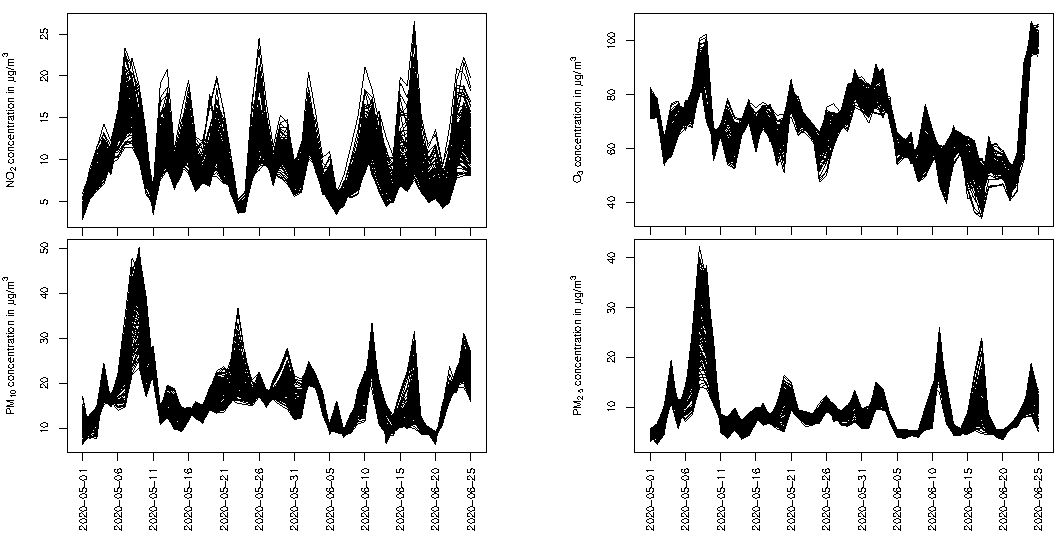
\includegraphics[width=\linewidth]{curves_real_data.pdf}
\caption{Daily concentration curves of $\text{NO}_2$, $\text{O}_3$, $\text{PM}_{10}$ and $\text{PM}_{2.5}$ (from May 1, 2020 to June 25, 2020) in each of the 169 \textit{cantons} of \textit{Nord-Pas-de-Calais} (a region in northern France). A marked temporal variability in the concentrations of the four pollutants is observed over the study period.}
\label{fig:description_curves}
\end{figure}
\begin{figure}[htbp]
\centering
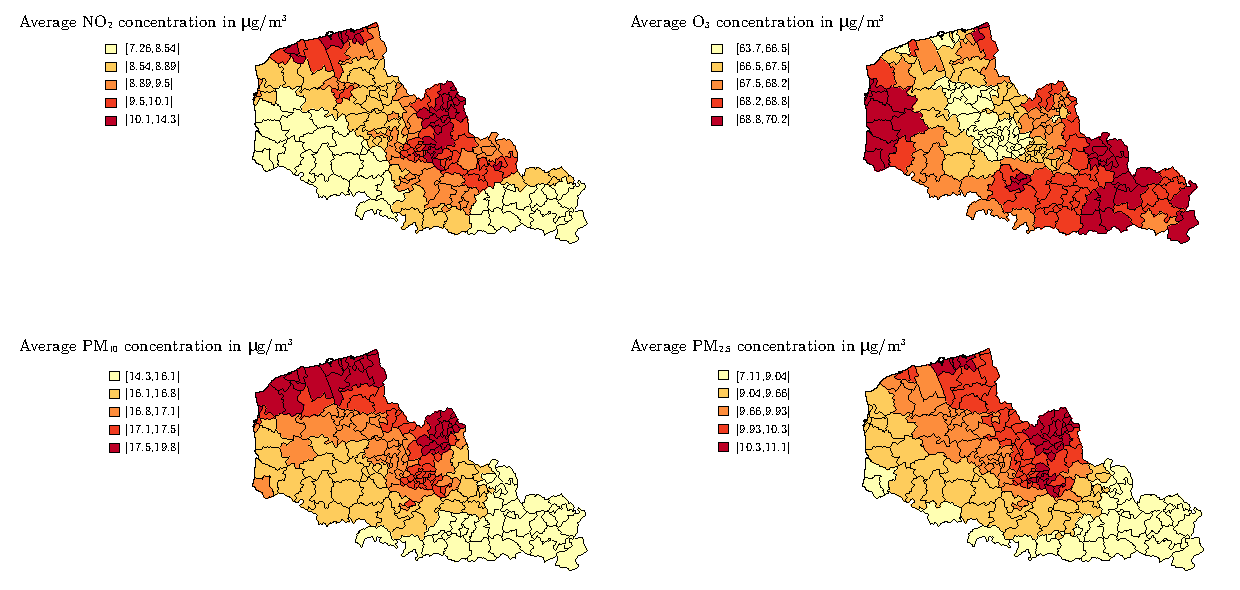
\includegraphics[width=\linewidth]{map_real_data.pdf}
\caption{Spatial distributions of the average concentrations of $\text{NO}_2$, $\text{O}_3$, $\text{PM}_{10}$ and $\text{PM}_{2.5}$ over the period from May 1, 2020 to June 25, 2020. A spatial heterogeneity of the average concentration (over the study period) is observed for the four pollutants. The spatial distributions of the average concentrations of $\text{PM}_{10}$ and $\text{PM}_{2.5}$ are also observed to be similar.}
\label{fig:description_mean}
\end{figure}

\noindent The maps in Figure~\ref{fig:description_mean} show a spatial heterogeneity of the average concentration for each pollutant.  Thus spatial scan statistics seem to be suitable to highlight the presence of \textit{cantons}-level spatial clusters of pollutants concentrations. 
Moreover since the curves in Figure~\ref{fig:description_curves} show a marked temporal variability during the period from May 1, 2020 to June 25, 2020 a functional approach is more appropriate. However for sake of completeness we will also perform a multivariate spatial scan statistic approach anyway.
Since small clusters of pollution are more relevant for interpretation because the sources of the pollutants are very localized, we will consider an \textit{a posteriori} filtering of maximum radius equal to 10 km.

\subsection{A multivariate spatial scan statistic} \label{subsec:resmulti}

First we will investigate a multivariate spatial scan statistic. In this example the temporal component of the multivariate functional data was suppressed by averaging the components over the time and we looked for spatial clusters of the combination of the different air pollutants. This will pick
up areas of multiple exposure to pollutants or, on the contrary, areas with little pollution. We first checked the normality of each variable, which has been done by using a histogram and a qqplot.
Since the distribution of the pollutants temporal mean concentrations is non-normal we decide to apply the MNP scan procedure. Here the system of coordinates is ``WGS84'', it must be filled with the argument \code{system}. As explained in Section~\nameref{subsec:computing}, \cite{spatialdisease} recommended to consider a maximum size of half the study region for the potential clusters so we use this \textit{a priori} filtering with the parameters \code{mini}, \code{maxi} and \code{type\_minimaxi}: the potential clusters are circular and they contain between 1 and 50\% of the sites. Then as noticed in Section~\nameref{subsec:airpollution}, we will apply an \textit{a posteriori} filtering of maximum radius equal to 10 km (arguments \code{mini\_post}, \code{maxi\_post} and \code{type\_minimaxi\_post}). Here we only want to consider the significant clusters at the 5\% threshold. Thus we leave the \code{typeI} parameter at its default value (0.05). However it should be noted that it is possible to obtain all the clusters (the MLC and the secondary clusters \citep{spatialscanstat}) by setting the \code{typeI} value at 1.

\begin{example}
 library(sp)
 coords <- coordinates(map_sites)
 res_mnp <- SpatialScan(method = "MNP", data = multi_data, sites_coord = coords, 
 + system = "WGS84", mini = 1, maxi = nrow(coords)/2, type_minimaxi = "sites/indiv", 
 + mini_post = 0, maxi_post = 10, type_minimaxi_post = "radius", 
 + nbCPU = 7, MC = 99, variable_names = c("NO2", "O3", "PM10", "PM2.5"))$MNP
\end{example}

\noindent Once the scan procedure is completed, the plot function can be used. For brevity, we only focus on the MLC and for the sake of completeness we will show the use of the three possible visualizations of the clusters. Since we have a spatial object \code{map\_sites} we can use the types \code{"map"} and \code{"map2"}. However for sake of completeness we also show the use of \code{"schema"} which allows to display the clusters otherwise (Figure~\ref{fig:mlc_mnp}). For the latter, since the system of the coordinates is ``WGS84'', the plot function requires to complete the parameter \code{system\_conv} which allows to correctly project the points. Here we choose the EPSG code 2154 corresponding to the Lambert 93 projection since the data is located in metropolitan France.

\begin{example}
 plot(x = res_mnp, type = "map", spobject = map_sites, only.MLC = TRUE)
 plot(x = res_mnp, type = "map2", spobject = map_sites, only.MLC = TRUE)
 plot(x = res_mnp, type = "schema", system_conv = "+init=epsg:2154", only.MLC = TRUE)
\end{example}

\begin{figure}[htbp]
\centering
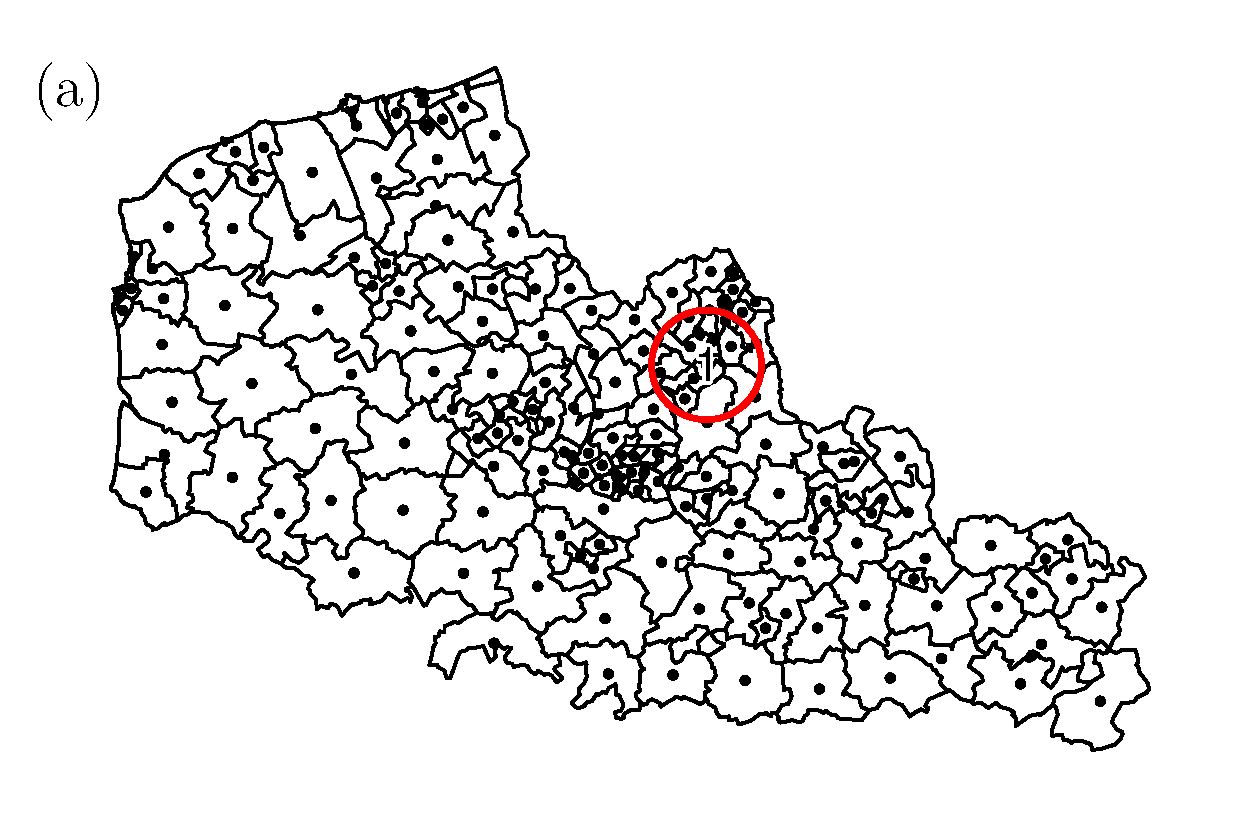
\includegraphics[width = 0.49\linewidth]{MLC_MNP_circle1.pdf}
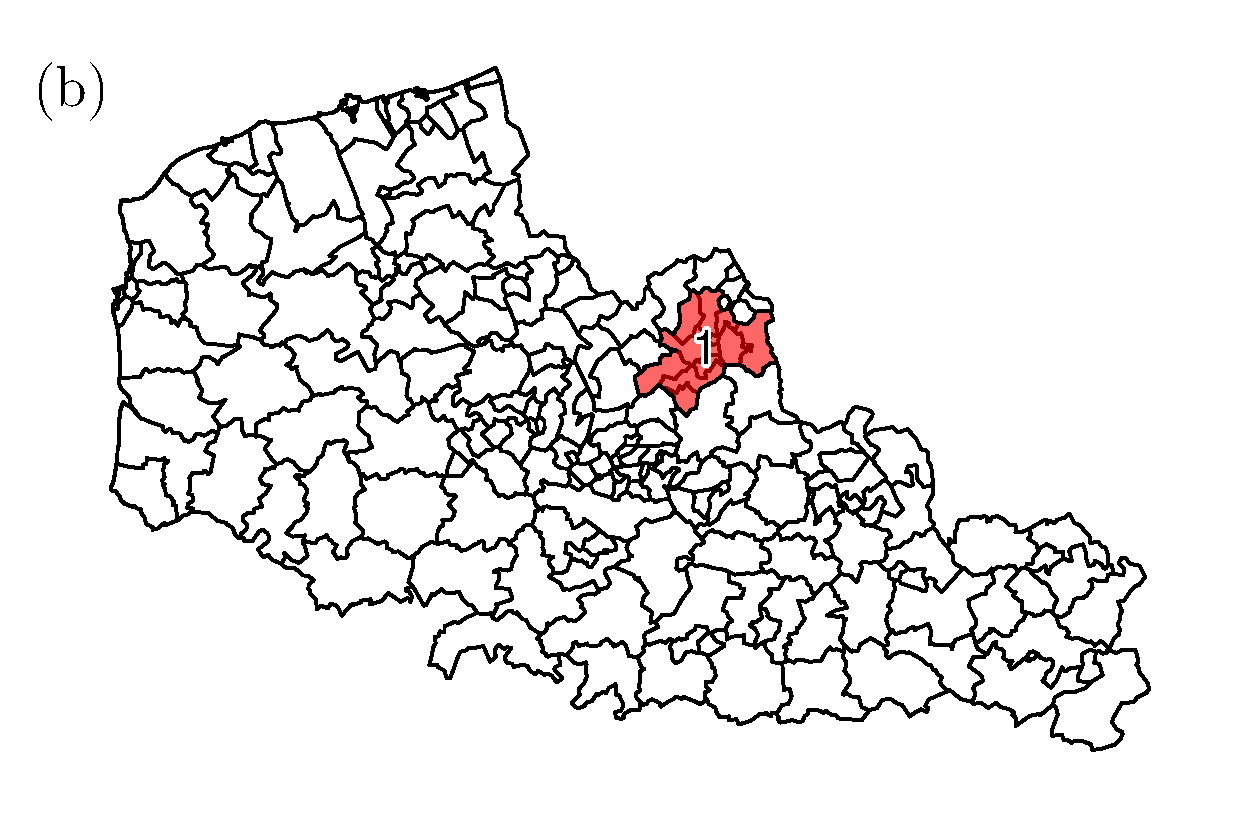
\includegraphics[width = 0.49\linewidth]{MLC_MNP1.pdf}
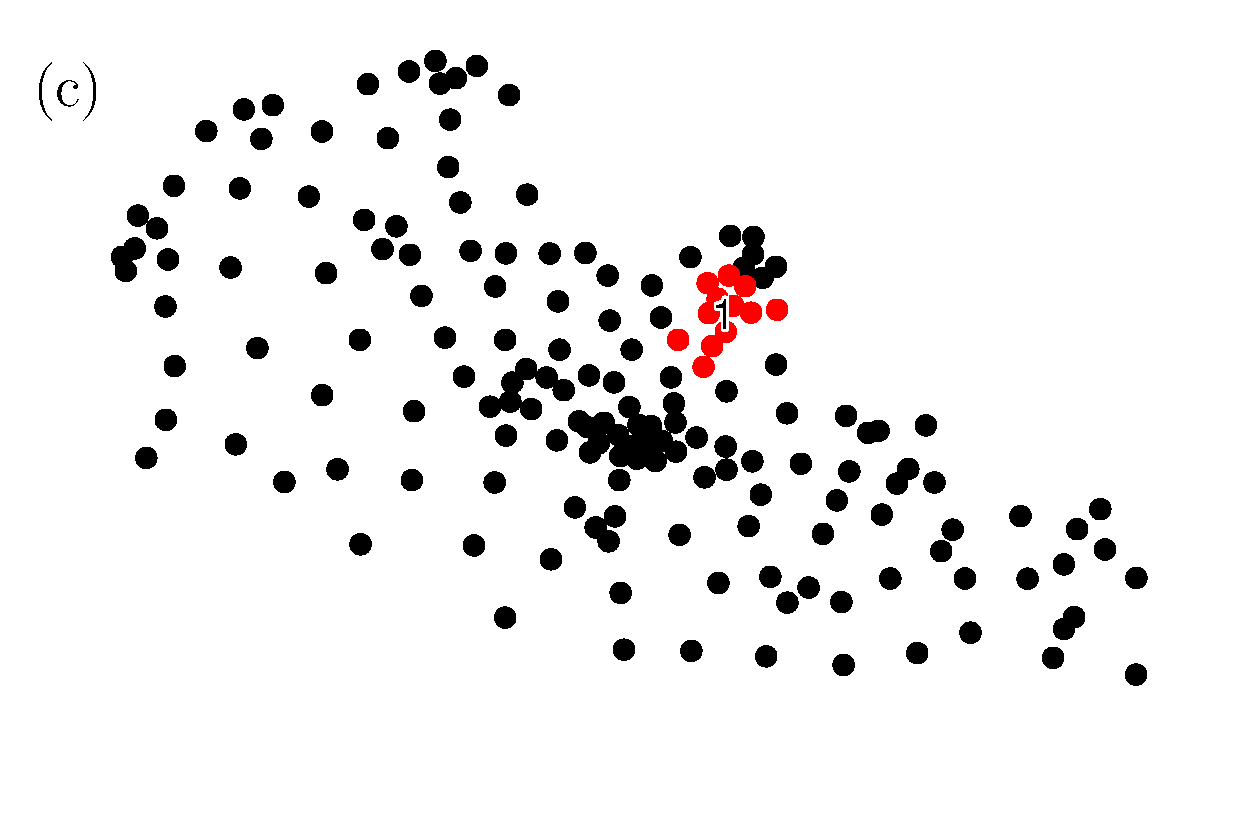
\includegraphics[width = 0.49\linewidth]{MLC_MNP_schema1.pdf}
\caption{Visualization of the most likely cluster with the function \code{plot} with the types \code{"map"} (panel a), \code{"map2"} (panel b) and \code{"schema"} (panel c) for the MNP scan procedure computed with the function \code{SpatialScan} on the average concentrations of $\text{NO}_2$, $\text{O}_3$, $\text{PM}_{10}$ and $\text{PM}_{2.5}$. The first two types of visualization require a spatial object corresponding to the spatial units (here the 169 \textit{cantons} of the \textit{Nord-Pas-de-Calais} region of northern France). The visualization option \code{"schema"} allows in the other case to draw a schema of the spatial units and the detected clusters. Here we focus the cluster visualization on the most likely cluster which is located in the urban area of Lille.}
\label{fig:mlc_mnp}
\end{figure}

\noindent Finally users may want to get some summarized characteristics, such as the quantiles of the variables. This can be achieved by using the function \code{summary} with the argument \code{type\_summ} equal to \code{"nparam"} (for the quantiles):


\begin{example}
 summary(res_mnp, type_summ = "nparam", only.MLC = TRUE)
\end{example}
\begin{example}
 ## $basic_summary
 ##         Cluster 1
 ## p-value     0.001
 ## Radius      9.999
 ## 
 ## $complete_summary
 ##                 Overall Inside cluster 1 Outside cluster 1
 ## Number of sites 169.000           12.000           157.000
 ## Q25 NO2           8.673           11.327             8.635
 ## Median NO2        9.183           11.721             9.075
 ## Q75 NO2           9.848           12.382             9.692
 ## Q25 O3           66.778           67.527            66.721
 ## Median O3        67.895           67.609            67.961
 ## Q75 O3           68.564           67.922            68.658
 ## Q25 PM10         16.397           17.483            16.205
 ## Median PM10      16.970           17.877            16.933
 ## Q75 PM10         17.372           17.962            17.266
 ## Q25 PM2.5         9.132           10.584             9.113
 ## Median PM2.5      9.833           10.678             9.790
 ## Q75 PM2.5        10.213           10.919            10.107
\end{example}


\noindent The user can also use the function \code{plotSummary} to display the spider chart corresponding to the detected cluster (Figure~\ref{fig:spiderchart}).

\begin{example}
 plotSummary(res_mnp, type = "median", only.MLC = TRUE)
\end{example}

\begin{figure}[htbp]
\centering
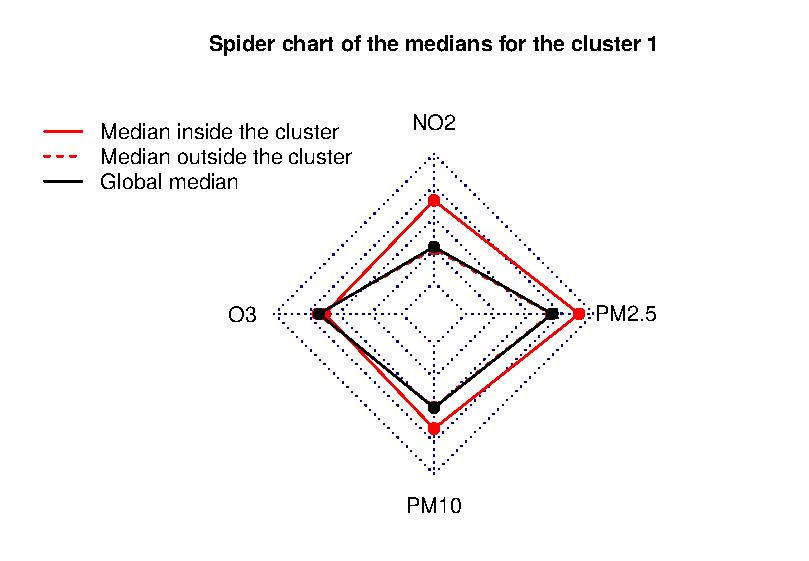
\includegraphics[width=0.6\linewidth]{MNP_spider_chart.pdf}
\caption{Spider chart obtained with the function \code{plotSummary} for the most likely cluster detected on the average concentrations of $\text{NO}_2$, $\text{O}_3$, $\text{PM}_{10}$ and $\text{PM}_{2.5}$ by the MNP scan procedure in northern France. The most likely cluster is characterized by larger median concentrations of $\text{NO}_2$, $\text{PM}_{10}$ and $\text{PM}_{2.5}$ than outside the cluster.}
\label{fig:spiderchart}
\end{figure}

\noindent The MLC is located in the area of Lille. The summary and Figure~\ref{fig:spiderchart} show that it is a cluster of overpollution (except for the pollutant $\text{O}_3$). %This result is consistent since it is well-known that the pollutants are more frequent in urban areas.
This cluster is especially characterized by high concentrations of $\text{NO}_2$ and $\text{PM}_{2.5}$ which indicates pollution from road traffic and from the residential sector (auxiliary heating in particular). As the adverse health effects of air pollution (and their potential synergistic effect) are well established, such a result could inform local stakeholders about immediate interventions around the area of Lille to reduce the air pollution levels.

\noindent We have obtained some first results however the curves on Figure~\ref{fig:description_curves} present a marked temporal variability during the study period. Thus it could be interesting to apply functional spatial scan statistics.

\subsection{A univariate functional spatial scan statistic}

Here we only consider the pollutant $\text{NO}_2$. Applying a spatial scan statistic for univariate functional data will thus allow to highlight areas where the $\text{NO}_2$ concentration curves are abnormally high or, on the contrary abnormally low. We choose to use the URBFSS scan procedure since it often presents higher powers and true positive rates than the other univariate functional methods as its multivariate counterpart MRBFSS \citep{notre_fonctionnel1}. As mentioned in Section~\nameref{subsec:resmulti} we decide to use the set of potential clusters \textit{a priori} in the Equation~\ref{eq:cluster} which corresponds to the recommended approach of \cite{spatialdisease}, and to the default values of the parameters \code{mini}, \code{maxi} and \code{type\_minimaxi} in the scan functions. We also set a maximum radius equal to 10 km \textit{a posteriori}.

\begin{example}
 res_urbfss <- SpatialScan(method = "URBFSS", data = funi_data, sites_coord = coords, 
 + system = "WGS84", mini = 1, maxi = nrow(coords)/2, type_minimaxi = "sites/indiv", 
 + mini_post = 0, maxi_post = 10, type_minimaxi_post = "radius", 
 + nbCPU = 7, MC = 99)$URBFSS
 plot(res_urbfss, type = "map2", spobject = map_sites, only.MLC = TRUE)
\end{example}

\begin{figure}[htbp]
\centering
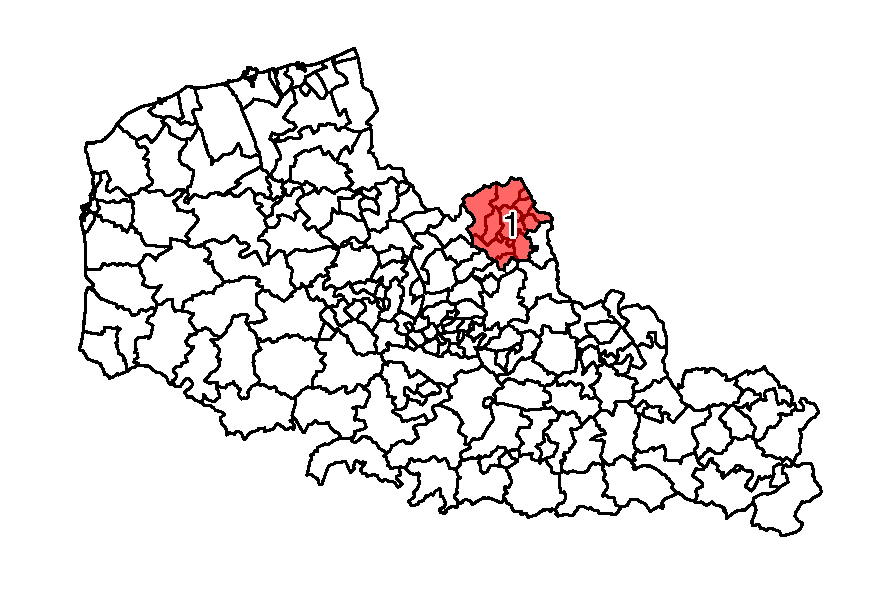
\includegraphics[width=0.49\linewidth]{MLC_urbfss.pdf}
\caption{Visualization of the detected clusters with the function \code{plot} with \code{type = "map2"} for the URBFSS scan procedure computed using the concentrations of $\text{NO}_2$ in the 169 \textit{cantons} of the \textit{Nord-Pas-de-Calais} region of northern France over the period from May 1, 2020 to June 25, 2020. Here we focus the cluster visualization on the most likely cluster which is located in the urban area of Lille.}
\label{fig:mlc_urbfss}
\end{figure}

\noindent Again the MLC is located in the area of Lille (Figure~\ref{fig:mlc_urbfss}). 

\noindent For functional data another function is provided to give some characteristics of the clusters: we can visualize the curves in the cluster by adding the curve of the global median with the function \code{plotCurves}. The function \code{plotSummary} allows to visualize the median curves inside and outside the cluster (Figure~\ref{fig:curves}): this is a cluster of overexposure to $\text{NO}_2$, which indicates traffic-related air pollution. Since exposure to pollution impacts health negatively, these results can be used to intervene to reduce air pollution.

\begin{example}
 plotCurves(res_urbfss, add_median = TRUE, only.MLC = TRUE)
 plotSummary(res_urbfss, type = "median", only.MLC = TRUE)
\end{example}

\begin{figure}[htbp]
\centering
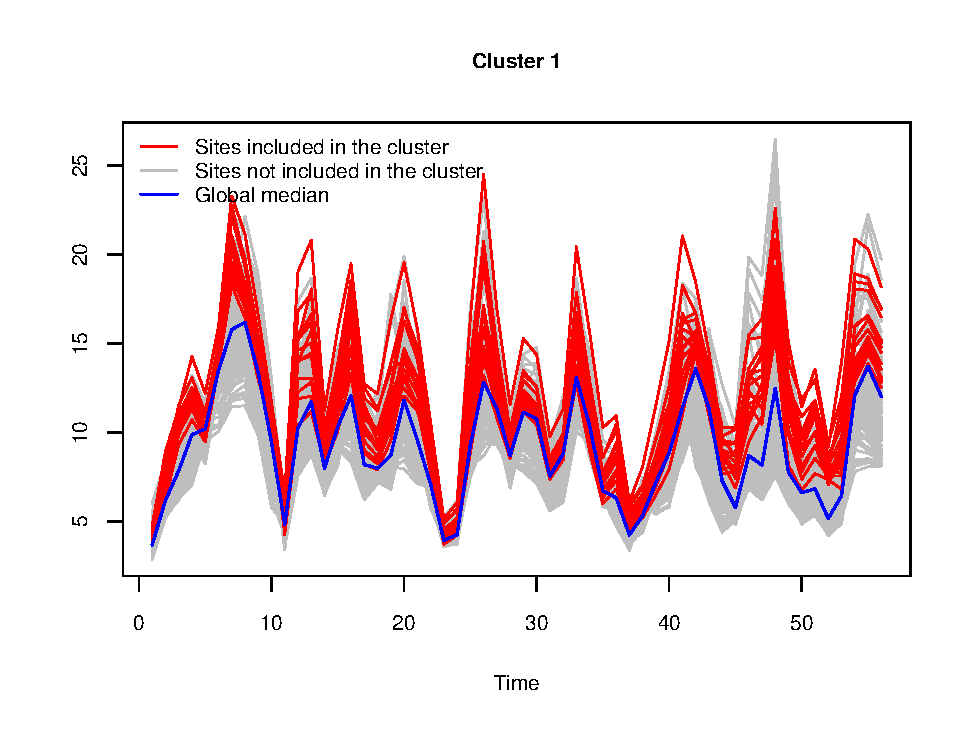
\includegraphics[width=0.49\linewidth]{curves_urbfss.pdf}
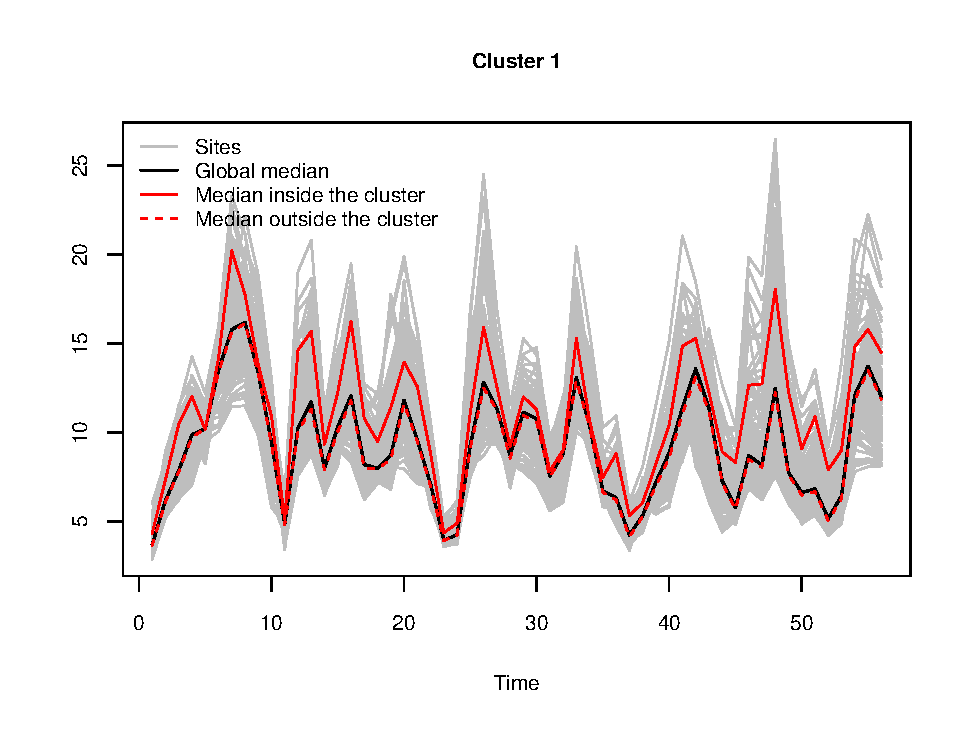
\includegraphics[width=0.49\linewidth]{summary_urbfss.pdf}
\caption{Characterization of the most likely cluster detected by the URBFSS scan approach in the context of univariate functional data consisting of the $\text{NO}_2$ concentrations in northern France over the period from May 1, 2020 to June 25, 2020 with the functions \code{plotCurves} (left panel) and \code{plotSummary} (right panel).
The most likely cluster is characterized by high concentration curves with a median concentration curve higher than outside the cluster.
}
\label{fig:curves}
\end{figure}

\subsection{A functional multivariate spatial scan statistic}

Now we consider the four pollutants together. To detect spatial clusters of the combination of the four pollutants considering all available information on the time period, we apply a spatial scan statistic for multivariate functional data. It will identify geographical areas in which one or more of the pollutant concentration curves are abnormally high or abnormally low. For the same reason that we have previously chosen to apply the URBFSS scan procedure, we use the MRBFSS in this context, with the same restrictions \textit{a priori} and \textit{a posteriori} as for the MNP and the URBFSS scan approaches.


\begin{example}
 res_mrbfss <- SpatialScan(method = "MRBFSS", data = fmulti_data, sites_coord = coords, 
 + system = "WGS84", mini = 1, maxi = nrow(coords)/2, type_minimaxi = "sites/indiv", 
 + mini_post = 0, maxi_post = 10, type_minimaxi_post = "radius", 
 + nbCPU = 7, MC = 99, variable_names = c("NO2", "O3", "PM10", "PM2.5"))$MRBFSS
 plot(res_mrbfss, type = "map2", spobject = map_sites, only.MLC = TRUE)
\end{example}

\begin{figure}[htbp]
\centering
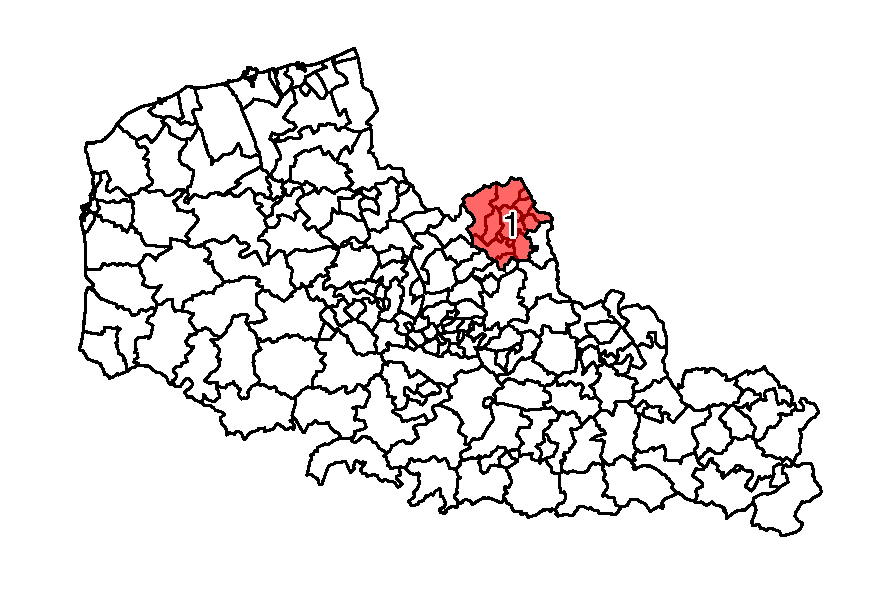
\includegraphics[width = 0.49\linewidth]{MLC_MRBFSS.pdf}
\caption{Visualization of the most likely cluster with the function \code{plot} with \code{type = "map2"} for the MRBFSS scan procedure computed using the concentrations of $\text{NO}_2$, $\text{O}_3$, $\text{PM}_{10}$ and $\text{PM}_{2.5}$ in the 169 \textit{cantons} of the \textit{Nord-Pas-de-Calais} region of northern France over the period from May 1, 2020 to June 25, 2020. The most likely cluster is located in the urban area of Lille.}
\label{fig:mlc_mrbfss}
\end{figure}

\noindent The detected cluster is exactly the same as before and is therefore located in the urban area of Lille (Figure~\ref{fig:mlc_mrbfss}).

\noindent Again we will display the curves in the cluster by adding the curve of the global median (Figure~\ref{fig:curves_multi}), as well as the median curves inside and outside the cluster which show that this is a cluster of high concentrations of $\text{NO}_2$, $\text{PM}_{10}$ and $\text{PM}_{2.5}$ (Figure~\ref{fig:summary_multi}). As mentioned in Section~\nameref{subsec:resmulti}, in environmental science it is well-known that $\text{NO}_2$ and $\text{PM}_{2.5}$ are more frequent in urban areas due to road traffic and population density so this is consistent with the cluster observed here. As the adverse health effects of air pollution and the combined effects of air pollutants are well established, this result could enable interventions by local authorities around the Lille area to reduce air pollution.

\begin{example}
 plotCurves(res_mrbfss, add_median = TRUE, only.MLC = TRUE)
 plotSummary(res_mrbfss, type = "median", only.MLC = TRUE)
\end{example}

\begin{figure}[htbp]
\centering
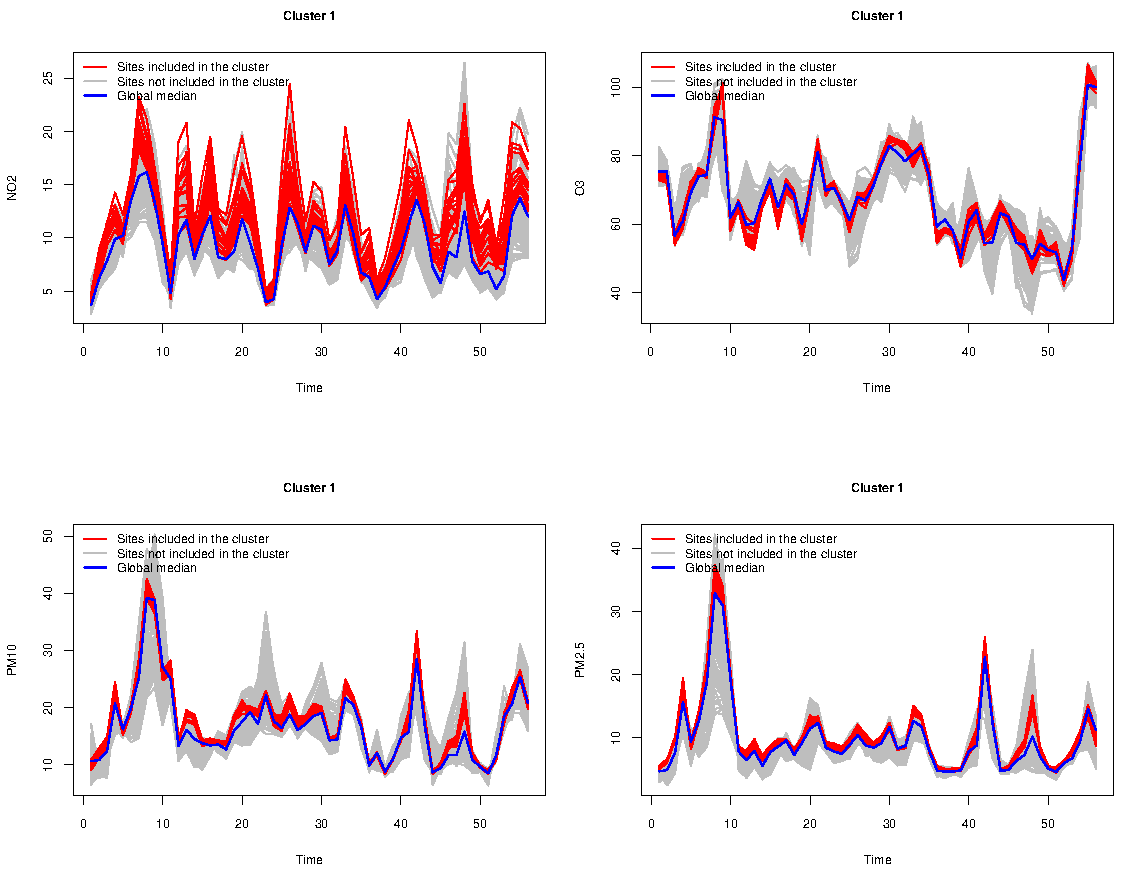
\includegraphics[width=\linewidth]{curves_mrbfss.pdf}
\caption{
Characterization of the most likely cluster detected by the MRBFSS scan approach in the context of multivariate functional data consisting of the $\text{NO}_2$, $\text{O}_3$, $\text{PM}_{10}$ and $\text{PM}_{2.5}$ concentrations in northern France over the period from May 1, 2020 to June 25, 2020 with the function \code{plotCurves}.
The most likely cluster is characterized by high concentration curves of $\text{NO}_2$, $\text{PM}_{10}$ and $\text{PM}_{2.5}$.
}
\label{fig:curves_multi}
\end{figure}

\begin{figure}[htbp]
\centering
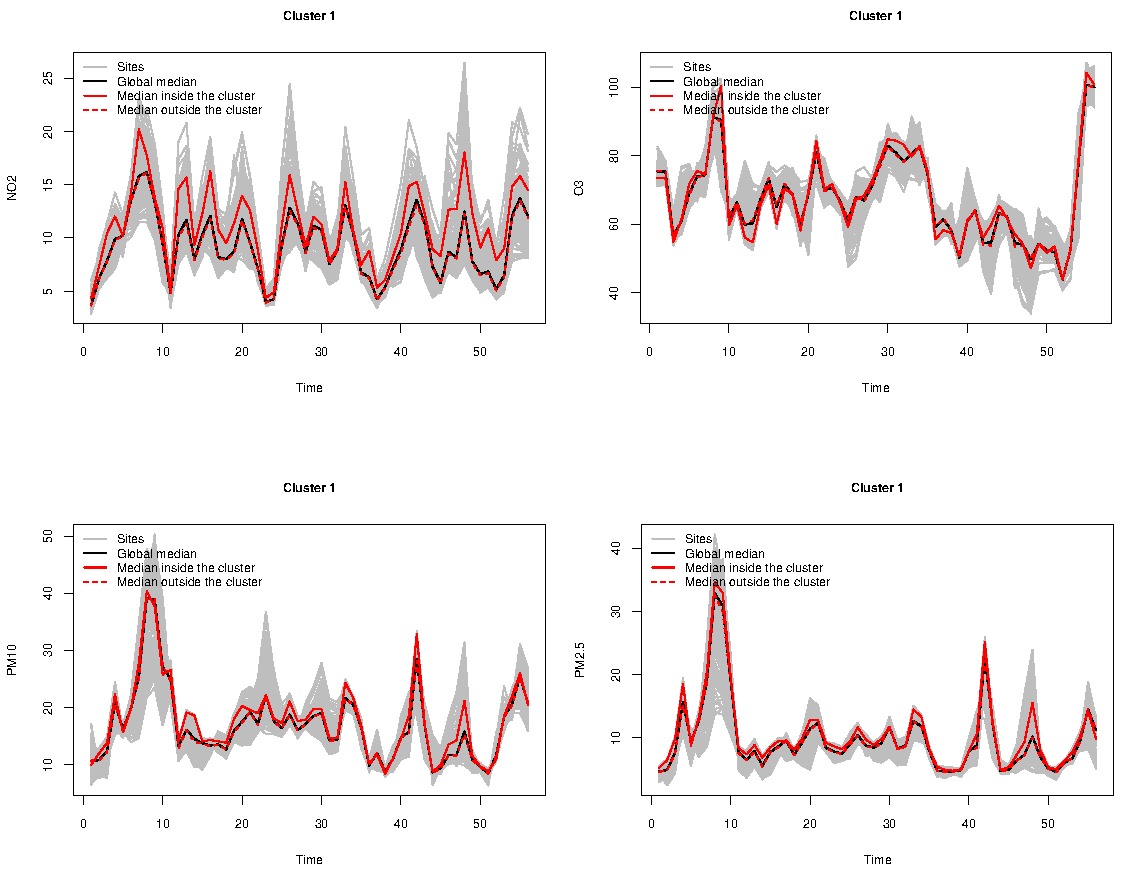
\includegraphics[width=\linewidth]{summary_mrbfss.pdf}
\caption{
Characterization of the most likely cluster detected by the MRBFSS scan approach in the context of multivariate functional data consisting of the $\text{NO}_2$, $\text{O}_3$, $\text{PM}_{10}$ and $\text{PM}_{2.5}$ concentrations in northern France over the period from May 1, 2020 to June 25, 2020 with the function \code{plotSummary}.
The most likely cluster is characterized by median concentration curves of $\text{NO}_2$, $\text{PM}_{10}$ and $\text{PM}_{2.5}$ higher than outside the cluster.
}
\label{fig:summary_multi}
\end{figure}



\section{Summary} \label{sec:conclusion}
In this article we presented the \pkg{HDSpatialScan} package. It makes it very easy to apply the existing scan statistics developed for multivariate data or functional data (univariate or multivariate), and the new rank-based scan statistic for univariate functional data presented in the Section~\nameref{sec:method}. 
The potential clusters considered are of variable size and circular.
In further updates of the package \pkg{HDSpatialScan} other shapes of scanning window such as elliptical or rectangular shapes will be implemented.
Our package also allows to easily plot and summarize the detected clusters. Then examples of applications of the functions of the package have been shown. \pkg{HDSpatialScan} presents the advantage that all the scan procedures are applied using the same function \code{SpatialScan} and it uses the classical R functions \code{plot}, \code{print} and \code{summary} which makes it very quick to get started.

% This file is only a basic article template. For full details of \emph{The R Journal} style and information on how to prepare your article for submission, see the \href{https://journal.r-project.org/share/author-guide.pdf}{Instructions for Authors}.

\bibliography{frevent}

\address{Camille Frévent\\
  University of Lille, CHU Lille,
  ULR 2694 - METRICS: Évaluation des technologies de santé et des pratiques médicales, INRIA‐MODAL \\
  F-59000 Lille
  France\\
  \email{camille.frevent@univ-lille.fr}}

\address{Mohamed-Salem Ahmed\\
  University of Lille, CHU Lille,
  ULR 2694 - METRICS: Évaluation des technologies de santé et des pratiques médicales \\
  F-59000 Lille
  France}

\address{Julien Soula\\
  University of Lille, CHU Lille,
  ULR 2694 - METRICS: Évaluation des technologies de santé et des pratiques médicales \\
  F-59000 Lille
  France}

\address{Lionel Cucala\\
  IMAG, Université de Montpellier, CNRS \\
  Montpellier \\
  France}

\address{Zaineb Smida\\
  IMAG, University of Montpellier, CNRS \\
  Montpellier \\
  France}

\address{Sophie Dabo-Niang\\
  Laboratoire Paul Painvelé UMR CNRS 8524, INRIA‐MODAL, University of Lille \\
  F-59000 Lille
  France}
  
\address{Michaël Genin\\
  University of Lille, CHU Lille,
  ULR 2694 - METRICS: Évaluation des technologies de santé et des pratiques médicales \\
  F-59000 Lille
  France}


